% \begin{lemma}
%     \label{antipattern:lem:leq_gamma_mono_x_l}
%     \ \newline
%     \noindent
%     \begin{minipage}{0.7\textwidth}\setlength{\parindent}{1em}
%     Let $\mathcal{X} = (X, f:X \rightarrowtail F)$ be a ruler-graph and \( \rho = (L \overset{l}{\leftarrowtail} K \overset{r}{\rightarrowtail} R) \) be a rule. Consider the DPO diagram illustrated on the right. 
% \end{minipage}%
% \begin{minipage}{0.29\textwidth}
%     \hfill
%     \begin{tikzpicture}
%         % [node distance=15mm]
%         \node (I) {$K$};
%         \node (L) [left of=I] {$L$};
%         \node (R) [right of=I] {$R$};
%         \node (G) [below of=L] {$G$};
%         \node (C) [below of=I] {$C$};
%         \node (H) [below of=R] {$H$}; 
%         \draw [>->] (I) to  node [midway,below] {$l$} (L);
%         \draw [>->] (I) to  node [midway,below] {$r$} (R);
%         \draw [>->] (L) to node [midway,right] {$m$} (G);
%         \draw [>->] (I) to  node [midway,right] {$u$} (C); 
%         \draw [>->] (R) to  node [midway,right] {$m'$} (H);
%         \draw [>->] (C) to node [midway,above] {$l'$} (G);
%         \draw [>->] (C) to node [midway,above] {$r'$} (H);
%         % \node [at=($(I)!.5!(G)$)] {\normalfont PO};
%         % \node [at=($(I)!.5!(H)$)] {\normalfont PO};
%       \end{tikzpicture}
% \end{minipage} 

% We have
%         $  \{
%              h_{XL} \in \operatorname{Mono}(\mathcal{X},L)_{\operatorname{NF}} \mid 
%              \exists h_{FG}. h_{XL} \star m = f \star h_{FG}
%          \}
%          \subseteq
%             \Gamma(\operatorname{Mono}(\mathcal{X},L)_{\operatorname{NF}})
%             $ 
% \end{lemma}
% \begin{proof}


% \todo{useful?}

%     By~\autoref{antipattern:def:gamma_l_rho_x} of $\Gamma$.
% \end{proof}

\begin{lemma}
    \label{antipattern:lem:xgm_xhmp_xl_xr_llsss}
     \ \newline
    \noindent
    \begin{minipage}{0.7\textwidth}\setlength{\parindent}{1em}
    Let $\mathcal{X} = (X, f:X \rightarrowtail F)$ be a ruler-graph and \( \rho = (L \overset{l}{\leftarrowtail} K \overset{r}{\rightarrowtail} R) \) be a rule. Consider the DPO diagram illustrated on the right. 
\end{minipage}%
\begin{minipage}{0.29\textwidth}
    \hfill
    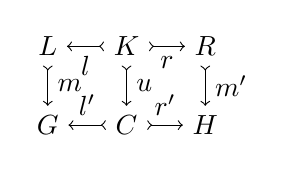
\begin{tikzpicture}
        % [node distance=15mm]
        \node (I) {$K$};
        \node (L) [left of=I] {$L$};
        \node (R) [right of=I] {$R$};
        \node (G) [below of=L] {$G$};
        \node (C) [below of=I] {$C$};
        \node (H) [below of=R] {$H$}; 
        \draw [>->] (I) to  node [midway,below] {$l$} (L);
        \draw [>->] (I) to  node [midway,below] {$r$} (R);
        \draw [>->] (L) to node [midway,right] {$m$} (G);
        \draw [>->] (I) to  node [midway,right] {$u$} (C); 
        \draw [>->] (R) to  node [midway,right] {$m'$} (H);
        \draw [>->] (C) to node [midway,above] {$l'$} (G);
        \draw [>->] (C) to node [midway,above] {$r'$} (H);
        % \node [at=($(I)!.5!(G)$)] {\normalfont PO};
        % \node [at=($(I)!.5!(H)$)] {\normalfont PO};
      \end{tikzpicture}
\end{minipage} 

We have
\begin{flalign*}
    \card{\operatorname{Mono}(\mathcal{X},G,m)_{\operatorname{NF}}} = 
    &\card{\operatorname{Mono}(\mathcal{X},L)_{\operatorname{NF}}} - 
    \\
    &\card{\{
                h_{XL} \in \operatorname{Mono}(\mathcal{X},L)_{\operatorname{NF}} \mid 
                \exists h_{FG}. h_{XL} \star m = f \star h_{FG}
            \}}
    \\
    \card{\operatorname{Mono}(\mathcal{X},H,m')_{\operatorname{NF}}} = 
    &\card{\operatorname{Mono}(\mathcal{X},R)_{\operatorname{NF}}} - 
    \\
    &\card{\{
                h_{XR} \in \operatorname{Mono}(\mathcal{X},R)_{\operatorname{NF}} \mid 
                \exists h_{FH}. h_{XR} \star m' = f \star h_{FH} 
                \}}
\end{flalign*}
\end{lemma}
\begin{proof}
    By symmetry, it suffices to prove the first equality and the second equality follows. To prove the first equality, we show that there is a bijection between $\operatorname{Mono}(\mathcal{X},G,m)_{\operatorname{NF}}$ and $\operatorname{Mono}(\mathcal{X},L)_{\operatorname{NF}} \setminus \{
                h_{XL} \in \operatorname{Mono}(\mathcal{X},L)_{\operatorname{NF}} \mid 
                \exists h_{FG}. h_{XL} \star m = f \star h_{FG}
            \}$.

    Let $h_{XG} \in \operatorname{Mono}(\mathcal{X},G,m)_{\operatorname{NF}}$.  By definition, there is a morphism $h_{XL}: X \rightarrowtail L$ such that $h_{XG} = h_{XL} \star m$ and no morphism $h_{FG}: F \rightarrowtail G$ such that $f \star h_{FG} = h_{XG}$. We must show $h_{XL} \in \operatorname{Mono}(\mathcal{X},L)_{\operatorname{NF}}$ and there is no $h_{FG}:f \rightarrowtail G$ such that $h_{XL} \star m = f \star h_{FG}$. These can be visualized by the following commutative diagram where edges that cannot exist are in red and dashed:

    \begin{center}
        \begin{tikzpicture}
            \node (k) at (0,1) {K};
            \node (l) at (-2,1) {L};
            \node (c) at (0,-1) {C};
            \node (g) at (-2,-1) {G};
            \node (x) at (-4,-3) {X};
            \node (f) at (-2,-3) {F};
            \draw[<-<]  (l) -- (k) node [midway,below] {l};
            \draw[>->] (c) -- (g) node [midway, above] {l'};
            \draw[>->] (l) -- (g) node[midway, right] {m};
            \draw[>->] (k) -- (c) node[midway, left] {};
            \draw[>->] (x) -- (g) node[midway,below] { };
            \draw[red,dashed,>->] (f) -- (g) node[midway] {$\times$};
            \draw[>->] (x) -- (l) node[midway,left] { };
            \draw[>->] (x) -- (f) node[midway,below] {$f$};
            \node () [at=($(l)!0.5!(c)$)] {PO};
        \end{tikzpicture}
    \end{center}
    
    We show $h_{XL} \in \operatorname{Mono}(\mathcal{X},L)_{\operatorname{NF}}$ by contradiction. Suppose that the contrary holds. There is a morphism $h_{FL}: F \rightarrowtail L$ such that $f \star h_{FL} = h_{XL}$.
    The image of $h_{XG}$ is, therefore, included in the image of $h_{FL} \star m$, as shown in the commutative diagram below, which contradicts the assumption that $h_{XG}$ is in $\operatorname{Mono}(\mathcal{X},G,m)_{\operatorname{NF}}$. 

    \begin{center}
        \begin{tikzpicture}
            \node (k) at (0,1) {K};
            \node (l) at (-2,1) {L};
            \node (c) at (0,-1) {C};
            \node (g) at (-2,-1) {G};
            \node (x) at (-4,-3) {X};
            \node (f) at (-4,-1) {F};
            \draw[<-<]  (l) -- (k) node [midway,below] {l};
            \draw[>->] (c) -- (g) node [midway, above] {l'};
            \draw[>->] (l) -- (g) node[midway, right] {m};
            \draw[>->] (k) -- (c) node[midway, left] {};
            \draw[>->] (x) -- (g) node[midway,below] { };
            \draw[>->] (f) -- (l) node[midway] {};
            \draw[>->] (x) -- (l) node[midway,left] { };
            \draw[>->] (x) -- (f) node[midway,left] {$f$};
            \node () [at=($(l)!0.5!(c)$)] {PO};
        \end{tikzpicture}
    \end{center}

    
    We show that there is no $h_{FG}:f \rightarrowtail G$ such that $h_{XL} \star m = f \star h_{FG}$ by contradiction. Suppose that the contrary holds. Under this assumption, we have the following commutative diagram. The image of $h_{XG}$ is, thus, included in the image of $f \star h_{FG}$ for some morphism $f$ which contradicts the assumption that $h_{XG}$ is in $\operatorname{Mono}(\mathcal{X},G,m)_{\operatorname{NF}}$.

    \begin{center}
        \begin{tikzpicture}
            \node (k) at (0,1) {K};
            \node (l) at (-2,1) {L};
            \node (c) at (0,-1) {C};
            \node (g) at (-2,-1) {G};
            \node (x) at (-4,-3) {X};
            \node (f) at (-2,-3) {F};
            \draw[<-<]  (l) -- (k) node [midway,below] {l};
            \draw[>->] (c) -- (g) node [midway, above] {l'};
            \draw[>->] (l) -- (g) node[midway, right] {m};
            \draw[>->] (k) -- (c) node[midway, left] {};
            \draw[>->] (x) -- (g) node[midway,below] { };
            \draw[>->] (f) -- (g) node[midway,right] {};
            \draw[>->] (x) -- (l) node[midway,left] { };
            \draw[>->] (x) -- (f) node[midway,below] {$f$};
            \node () [at=($(l)!0.5!(c)$)] {PO};
        \end{tikzpicture}
    \end{center}

    Let $h_{XG}, h_{XG}' \in \operatorname{Mono}(\mathcal{X},G,m)_{\operatorname{NF}}$ such that $h_{XG} \neq h_{XG}'$.  By definition, there are morphisms $h_{XL}, h_{XL}': X \rightarrowtail L$ such that $h_{XG} = h_{XL} \star m$, $h_{XG}' = h_{XL}' \star m$, and no morphism $h_{FG}, h_{FG}': F \rightarrowtail G$ such that $f \star h_{FG} = h_{XG}$ and $f \star h_{FG}' = h_{XG}'$. Since $m$ is injection, we have $h_{XL} \neq h_{XL}'$.

    There is, thus, an injection from $\operatorname{Mono}(\mathcal{X},G,m)_{\operatorname{NF}}$ to $\operatorname{Mono}(\mathcal{X},L)_{\operatorname{NF}} \setminus \{
                h_{XL} \in \operatorname{Mono}(\mathcal{X},L)_{\operatorname{NF}} \mid 
                \exists h_{FG}. h_{XL} \star m = f \star h_{FG}
            \}$.

    Conversely, let $h_{XL}$ be a morphism in $\operatorname{Mono}(\mathcal{X},L)_{\operatorname{NF}}\setminus \{
                h_{XL} \in \operatorname{Mono}(\mathcal{X},L)_{\operatorname{NF}} \mid 
                \exists h_{FG}. h_{XL} \star m = f \star h_{FG}
            \}$. 
    We have the following commutative diagram:
    
    \begin{center}
        \begin{tikzpicture}
            \node (k) at (0,1) {K};
            \node (l) at (-2,1) {L};
            \node (c) at (0,-1) {C};
            \node (g) at (-2,-1) {G};
            \node (x) at (-4,-3) {X};
            \node (f) at (-4,-1) {F};
            \draw[<-<]  (l) -- (k) node [midway,below] {l};
            \draw[>->] (c) -- (g) node [midway, above] {l'};
            \draw[>->] (l) -- (g) node[midway, right] {m};
            \draw[>->] (k) -- (c) node[midway, left] {};
            \draw[red,dashed,>->] (f) -- (l) node[midway] {$\times$};
            \draw[>->] (x) -- (l) node[midway,left] { };
            \draw[>->] (x) -- (f) node[midway,left] {f};
            \draw[red,dashed,>->] (f) -- (g) node[pos=0.75] {$\times$};
            \node () [at=($(l)!0.5!(c)$)] {PO};
        \end{tikzpicture}
    \end{center}
    To prove $h_{XL} \star m \in \operatorname{Mono}(\mathcal{X},G,m)_{\operatorname{NF}}$, we show that we have $h_{XL} \star m \in \operatorname{Mono}(\mathcal{X},G,m)$ and that there is no morphism $h_{FG}: F \rightarrowtail G$ such that $f \star h_{FG} = h_{XL} \star m$. We have $h_{XL} \star m \in \operatorname{Mono}(\mathcal{X},G,m)$, because $h_{XL} \star m = f \star h_{FG}$, by definition. There is no morphism $h_{FG}: F \rightarrowtail G$ such that $f \star h_{FG} = h_{XL} \star m$, by definition of $h_{XL}$.

    Let $h_{XL}, h_{XL}'$ be morphisms in $\operatorname{Mono}(\mathcal{X},L)_{\operatorname{NF}}\setminus \{
                h_{XL} \in \operatorname{Mono}(\mathcal{X},L)_{\operatorname{NF}} \mid 
                \exists h_{FG}. h_{XL} \star m = f \star h_{FG}
            \}$ such that $h_{XL} \neq h_{XL}'$.
    Since $m$ is injective, we have $h_{XL} \star m \neq h_{XL}' \star m$. 

    There is, thus, an injection from $(\operatorname{Mono}(\mathcal{X},L)_{\operatorname{NF}}\setminus \{
                h_{XL} \in \operatorname{Mono}(\mathcal{X},L)_{\operatorname{NF}} \mid 
                \exists h_{FG}. h_{XL} \star m = f \star h_{FG}
            \}) \star m$ to $\operatorname{Mono}(\mathcal{X},G,m)_{\operatorname{NF}}$. Since $(\operatorname{Mono}(\mathcal{X},L)_{\operatorname{NF}}\setminus \{
                h_{XL} \in \operatorname{Mono}(\mathcal{X},L)_{\operatorname{NF}} \mid 
                \exists h_{FG}. h_{XL} \star m = f \star h_{FG}
            \}) \star m$ and $\operatorname{Mono}(\mathcal{X},L)_{\operatorname{NF}}\setminus \{
                h_{XL} \in \operatorname{Mono}(\mathcal{X},L)_{\operatorname{NF}} \mid 
                \exists h_{FG}. h_{XL} \star m = f \star h_{FG}
            \}$ are in bijection, we conclude that there is an injection from $\operatorname{Mono}(\mathcal{X},L)_{\operatorname{NF}}\setminus \{
                h_{XL} \in \operatorname{Mono}(\mathcal{X},L)_{\operatorname{NF}} \mid 
                \exists h_{FG}. h_{XL} \star m = f \star h_{FG}
            \}$ to $\operatorname{Mono}(\mathcal{X},G,m)_{\operatorname{NF}}$.

    Finally, we conclude.
\end{proof}



\noindent
\begin*{\textbf{\autoref{antipattern:lem:xgm_xhmp_xl_xr}}}
    \newline
    \noindent
\begin{minipage}{0.7\textwidth}\setlength{\parindent}{1em}
    Let $\mathcal{X}$
    % $\mathcal{X} = (X, f:X \rightarrowtail F)$
     be a ruler-graph and \( \rho = (L \overset{l}{\leftarrowtail} K \overset{r}{\rightarrowtail} R) \) be a rule. Consider the DPO diagram illustrated on the right. 
\end{minipage}%
\begin{minipage}{0.29\textwidth}
    \hfill
    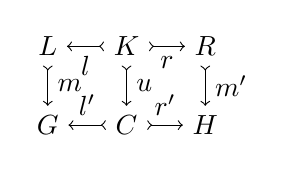
\begin{tikzpicture}
        % [node distance=15mm]
        \node (I) {$K$};
        \node (L) [left of=I] {$L$};
        \node (R) [right of=I] {$R$};
        \node (G) [below of=L] {$G$};
        \node (C) [below of=I] {$C$};
        \node (H) [below of=R] {$H$}; 
        \draw [>->] (I) to  node [midway,below] {$l$} (L);
        \draw [>->] (I) to  node [midway,below] {$r$} (R);
        \draw [>->] (L) to node [midway,right] {$m$} (G);
        \draw [>->] (I) to  node [midway,right] {$u$} (C); 
        \draw [>->] (R) to  node [midway,right] {$m'$} (H);
        \draw [>->] (C) to node [midway,above] {$l'$} (G);
        \draw [>->] (C) to node [midway,above] {$r'$} (H);
        % \node [at=($(I)!.5!(G)$)] {\normalfont PO};
        % \node [at=($(I)!.5!(H)$)] {\normalfont PO};
      \end{tikzpicture}
\end{minipage} 

We have 
    $$
        \card{\operatorname{Mono}(\mathcal{X},G,m)_{\operatorname{NF}}} - 
        \card{\operatorname{Mono}(\mathcal{X},H,m')_{\operatorname{NF}}} \geq
        \Lambda(\mathcal{X}, \rho)
    $$
    where $\Lambda(\mathcal{X},\rho) \overset{\operatorname{def}}{=} \card{\operatorname{Mono}(\mathcal{X},L)_{\operatorname{NF}}} - 
    \card{\Gamma(\operatorname{Mono}(\mathcal{X},L)_{\operatorname{NF}})} -
   \card{\operatorname{Mono}(\mathcal{X},R)_{\operatorname{NF}}}$.
\end*{}

\begin{proof}
    \label{antipattern:proof:lem:xgm_xhmp_xl_xr}
    There are two cases to consider: either $\mathcal{X}=(X)$ or $\mathcal{X}=(X,f:X \rightarrowtail F)$. For the first case, since $\Gamma(\operatorname{Mono}(\mathcal{X},L)_{\operatorname{NF}}) = \emptyset$ by definition, the inequality is equivalent to the following:
    $$
        \card{\operatorname{Mono}(\mathcal{X},G,m)_{\operatorname{NF}}} - 
        \card{\operatorname{Mono}(\mathcal{X},H,m')_{\operatorname{NF}}} \geq
        \card{\operatorname{Mono}(\mathcal{X},L)_{\operatorname{NF}}} - 
        \card{\operatorname{Mono}(\mathcal{X},R)_{\operatorname{NF}}}
    $$
    By definition, it is equivalent to the following inequality:
    \begin{flalign*}
        \card{\operatorname{Mono}(X,G,m)} - 
        \card{\operatorname{Mono}(X,H,m')} \geq  
        \card{\operatorname{Mono}(X,L)} - 
   \card{\operatorname{Mono}(X,R)}
    \end{flalign*}
    which is true because $\card{\operatorname{Mono}(X,G,m)} = \card{\operatorname{Mono}(X,L)}$ and $\card{\operatorname{Mono}(X,H,m')} =
   \card{\operatorname{Mono}(X,R)}$ by~\autoref{subgraph_counting:lem:decomp_w_u}.
   
   For the second case, by~\autoref{antipattern:lem:xgm_xhmp_xl_xr_llsss}, we have the following:
    \begin{flalign*}
        &\card{\operatorname{Mono}(\mathcal{X},G,m)_{\operatorname{NF}}} - 
        \card{\operatorname{Mono}(\mathcal{X},H,m')_{\operatorname{NF}}} 
        \\
        = &(\card{\operatorname{Mono}(\mathcal{X},L)_{\operatorname{NF}}} - 
            \card{\{
                h_{XL} \in \operatorname{Mono}(\mathcal{X},L)_{\operatorname{NF}} \mid 
                \exists h_{FG}. h_{XL} \star m = f \star h_{FG}
            \}}
        ) - 
        \\
            &
           (
            \card{\operatorname{Mono}(\mathcal{X},R)_{\operatorname{NF}}}
            -  
            \card{\{
                h_{XR} \in \operatorname{Mono}(\mathcal{X},R)_{\operatorname{NF}} \mid 
                \exists h_{FH}. h_{XR} \star m' = f \star h_{FH}
            \}}
           )
    \end{flalign*}
    where 
    $\{
                h_{XL} \in \operatorname{Mono}(\mathcal{X},L)_{\operatorname{NF}} \mid 
                \exists h_{FG}. h_{XL} \star m = h_{XF} \star h_{FG}
            \}$ is the set of $X$-occurrences in $L$ that are not included in any occurrences of its forbidden context in $L$ but included in an occurrence of its forbidden context in $G$, and, analyogously, $\{
                h_{XR} \in \operatorname{Mono}(\mathcal{X},R)_{\operatorname{NF}} \mid 
                \exists h_{FH}. h_{XR} \star m' = h_{XF} \star h_{FH}
            \}$ is the set of $X$-occurrences in $R$ that are not included in any occurrences of its forbidden context in $R$ but included in an occurrence of its forbidden context in $H$.

    The following equalities and inequalities hold:
    \begin{flalign*}
        &\card{\operatorname{Mono}(\mathcal{X},G,m)_{\operatorname{NF}}} - 
        \card{\operatorname{Mono}(\mathcal{X},H,m')_{\operatorname{NF}}} 
        \\
           = &(\card{\operatorname{Mono}(\mathcal{X},L)_{\operatorname{NF}}} - 
           \card{\operatorname{Mono}(\mathcal{X},R)_{\operatorname{NF}}}
       ) + 
       \\
           &
          (
            \card{\{
               h_{XR} \in \operatorname{Mono}(\mathcal{X},R)_{\operatorname{NF}} \mid 
               \exists h_{FH}. h_{XR} \star m' = f \star h_{FH}
           \}}
           - \\&
           \card{\{
                h_{XL} \in \operatorname{Mono}(\mathcal{X},L)_{\operatorname{NF}} \mid 
                \exists h_{FG}. h_{XL} \star m = f \star h_{FG}
            \}}         
          ) 
        \\ 
        \geq& (\card{\operatorname{Mono}(\mathcal{X},L)_{\operatorname{NF}}} - 
        \card{\operatorname{Mono}(\mathcal{X},R)_{\operatorname{NF}}}
        ) -
        % \\
        % &
        %  0 -
         \\
         & \card{\{
             h_{XL} \in \operatorname{Mono}(\mathcal{X},L)_{\operatorname{NF}} \mid 
             \exists h_{FG}. h_{XL} \star m = h_{XF} \star h_{FG}
         \}}        
       \\ 
       =& (\card{\operatorname{Mono}(\mathcal{X},L)_{\operatorname{NF}}} - 
       \card{\operatorname{Mono}(\mathcal{X},R)_{\operatorname{NF}}}
       ) - 
       \\
       &
    %   (
    %     0 \mathop{-}   
       \card{
        \Gamma(\operatorname{Mono}(\mathcal{X},L)_{\operatorname{NF}})
        }      
    %   )  
        \text{\hspace{1cm}by~\autoref{antipattern:def:gamma_l_rho_x}}
      \\
      \mathop{=}& 
      \card{\operatorname{Mono}(\mathcal{X},L)_{\operatorname{NF}}} - 
      \card{
        \Gamma(\operatorname{Mono}(\mathcal{X},L)_{\operatorname{NF}})
        } \mathop{-}
      \card{\operatorname{Mono}(\mathcal{X},R)_{\operatorname{NF}}}
      \\
      =& \Lambda(\mathcal{X}, \rho)
    \end{flalign*}
\end{proof}

\begin{lemma}
    \label{antipattern:lem:xh_decomp}
     Consider the following pushout diagram in the category \textbf{Graph}:
     \begin{center}
        \begin{tikzpicture}
            \node (k) at (0,1) {K};
            \node (r) at (2,1) {R};
            \node (c) at (0,-1) {C};
            \node (h) at (2,-1) {H};
            \draw[>->]  (k) -- (r) node [midway,below] {r};
            \draw[>->] (c) -- (h) node [midway,above] {r'};
            \draw[>->] (r) -- (h) node[midway, left] {m'};
            \draw[>->] (k) -- (c) node[midway, left] {};
            \node () [at=($(r)!0.5!(c)$)] {PO};
        \end{tikzpicture}
    \end{center}
    Let $X$ be a graph, and $h_{XH}:X \rightarrowtail H$ a monomorphism. Then, we can construct the following commutative diagram in the category \textbf{Graph}: 

    \begin{center}
        \resizebox{0.3\textwidth}{!}{
            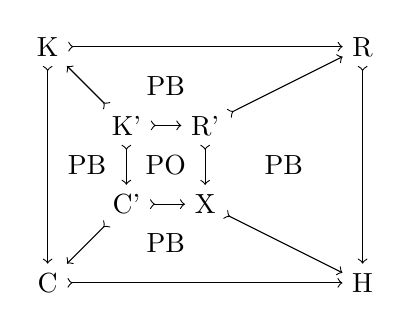
\begin{tikzpicture}
                \node (k) at (0,0) {K};
                \node (r) at (4,0) {R};
                \node (c) at (0,-3) {C};
                \node (h) at (4,-3) {H};
                \draw[<-<]  (r) -- (k) node [midway,above] {};
                \draw[>->] (c) -- (h) node [midway, below] {};
                \draw[>->] (r) -- (h) node[midway, left] {};
                \draw[>->] (k) -- (c) node[midway, left] {};
                \node (k') at (1,-1) {K'};
                \node (r') at (2,-1) {R'};
                \node (c') at (1,-2) {C'};
                \node () at (1.5,-1.5) {PO};
                \node () at (3,-1.5) {PB};
                \node () at (1.5,-2.5) {PB};
                \node () at (1.5,-0.5) {PB};
                \node () at (0.5,-1.5) {PB};
                \node (x) at (2,-2) {X};
                \draw [>->] (c') -- (x);
                \draw [>->] (r') -- (x);
                \draw [>->] (k') -- (r');
                \draw [>->] (k') -- (c');
                \draw [>->] (c') -- (c);
                \draw[>->] (r') -- (r);
                \draw[>->] (x) -- (h) node[midway,right] {};
                \draw[>->] (k') -- (k) ;
            \end{tikzpicture}
        }
        \end{center} 
\end{lemma}
\begin{proof}    
         In the category \textbf{Graph}, we can construct the following commutative diagram \todo{should I give more details?}:
        \begin{center}
            \resizebox{0.3\textwidth}{!}{
                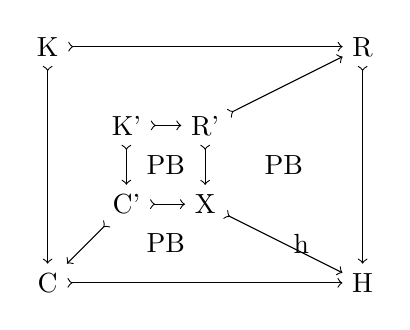
\begin{tikzpicture}
                    \node (k) at (0,0) {K};
                    \node (r) at (4,0) {R};
                    \node (c) at (0,-3) {C};
                    \node (h) at (4,-3) {H};
                    % \node (rb) at ($\scl*(1.5,-0.5)$) {$R_X$};
                    
                    % \node (h') at ($\scl*(1.5,-1.5)$) {$H'$};
                    % \draw[>->]  (rb) -- (h') node [midway,above] {};
                    % \draw[>->]  (c) -- (h') node [midway,above] {};
        
                    \draw[<-<]  (r) -- (k) node [midway,above] {};
                    \draw[>->] (c) -- (h) node [midway, below] {};
                    \draw[>->] (r) -- (h) node[midway, left] {};
                    \draw[>->] (k) -- (c) node[midway, left] {};
        
                    % \draw[->] (rb) to (l);
                    % \draw[<-<] (rb) to (k);
                
                    \node (k') at (1,-1) {K'};
                    \node (r') at (2,-1) {R'};
                    \node (c') at (1,-2) {C'};
                    \node () at (1.5,-1.5) {PB};
                    \node () at (3,-1.5) {PB};
                    \node () at (1.5,-2.5) {PB};
                    \node (x) at (2,-2) {X};
                    % \draw [->] (x) -- (h') node[midway] {!};
                    \draw [>->] (c') -- (x);
                    \draw [>->] (r') -- (x);
                    \draw [>->] (k') -- (r');
                    \draw [>->] (k') -- (c');
                    \draw [>->] (c') -- (c);
                    % \draw [->] (r') -- (rb);
                    % \draw [->] (r') -- (rb);
                    % \draw [->] (h') -- (h);
        
                    \draw[>->] (r') -- (r);
                    \draw[>->] (x) -- (h) node[midway,right] {h};
                    % \node (rb) at ($\scl*(\sclx*1.5,-0.5)$) {$R_X$};
                    % \node (h') at ($\scl*(\sclx*1.5,-1.2)$) {$H'$};
                    % \draw[>->]  (rb) -- (h') node [midway,above] {};
                    % \draw[>->]  (c) -- (h') node [midway,above] {};
                    % \draw[>->]  (rb) -- (h') node [midway,above] {};
                    % \draw[>->] (rb) to (r);
                    % \draw[<-<] (rb) to (k);
                \end{tikzpicture}
            }
            \end{center} 
        
        Since $KCHR$ is a pushout, it is also a pullback, by~\autoref{prop:pb_eq_po}. 
        Therefore, from \(
            h_{K'C'} \star h_{C'C} \star h_{CH} =h_{K'R'} \star h_{R'R} \star h_{R'R}
        \) and the universal property of pullback, there exists a unique morphism $h_{K'K}:K' \rightarrowtail K$ such that 
        \begin{flalign*}
            h_{K'C'} \star h_{C'C} &= h_{K'K} \star h_{KC} 
            % \label{antipattern:kpcpcpckpkkc}
            \\
            h_{K'R'} \star h_{R'R} &= h_{K'K} \star h_{KR} 
            % \label{antipattern:kprprprkpk}
         \end{flalign*}
        The square $K'KCC'$ and $K'R'RK$ are pullbacks, by~\autoref{kpcpck_pullback}. Furthermore, $K'C'XR'$ is a pushout by~\autoref{kpcpxrp_po}. Hence, the following commutative diagram holds:
        \begin{center}
            \resizebox{0.3\textwidth}{!}{
                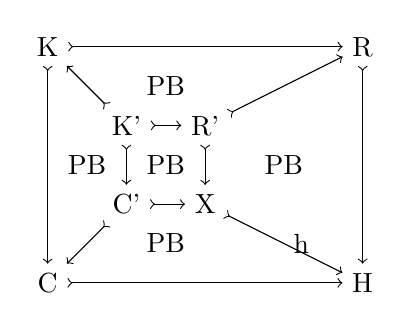
\begin{tikzpicture}
                    \node (k) at (0,0) {K};
                    \node (r) at (4,0) {R};
                    \node (c) at (0,-3) {C};
                    \node (h) at (4,-3) {H};
                    % \node (rb) at ($\scl*(1.5,-0.5)$) {$R_X$};
                    % \node (h') at ($\scl*(1.5,-1.5)$) {$H'$};
                    % \draw[>->]  (rb) -- (h') node [midway,above] {};
                    % \draw[>->]  (c) -- (h') node [midway,above] {};
                    \draw[<-<]  (r) -- (k) node [midway,above] {};
                    \draw[>->] (c) -- (h) node [midway, below] {};
                    \draw[>->] (r) -- (h) node[midway, left] {};
                    \draw[>->] (k) -- (c) node[midway, left] {};
                    % \draw[->] (rb) to (l);
                    % \draw[<-<] (rb) to (k);
                    \node (k') at (1,-1) {K'};
                    \node (r') at (2,-1) {R'};
                    \node (c') at (1,-2) {C'};
                    \node () at (1.5,-1.5) {PB};
                    \node () at (3,-1.5) {PB};
                    \node () at (1.5,-2.5) {PB};
                    \node () at (1.5,-0.5) {PB};
                    \node () at (0.5,-1.5) {PB};
                    \node (x) at (2,-2) {X};
                    % \draw [->] (x) -- (h') node[midway] {!};
                    \draw [>->] (c') -- (x);
                    \draw [>->] (r') -- (x);
                    \draw [>->] (k') -- (r');
                    \draw [>->] (k') -- (c');
                    \draw [>->] (c') -- (c);
                    % \draw [->] (r') -- (rb);
                    % \draw [->] (r') -- (rb);
                    % \draw [->] (h') -- (h);
                    \draw[>->] (r') -- (r);
                    \draw[>->] (x) -- (h) node[midway,right] {h};
                    % \node (rb) at ($\scl*(\sclx*1.5,-0.5)$) {$R_X$};
                    % \node (h') at ($\scl*(\sclx*1.5,-1.2)$) {$H'$};
                    % \draw[>->]  (rb) -- (h') node [midway,above] {};
                    % \draw[>->]  (c) -- (h') node [midway,above] {};
                    % \draw[>->]  (rb) -- (h') node [midway,above] {};
                    % \draw[>->] (rb) to (r);
                    % \draw[<-<] (rb) to (k);
                    \draw[>->] (k') -- (k) ;
                \end{tikzpicture}
            }
            \end{center} 
        \todo{use: assumption: non increasing}
        % Since the rule is by assumption $X$-non-increasing, there is a morphism $h_{R'L}$ such that $K'KLR'$ is commutative.
\end{proof}

\noindent
\begin*{\textbf{\autoref{lem:xglnotmlp_xhlnotmrp}}}
    \newline
    \noindent
    \vspace{2mm}
    \begin{minipage}{0.7\textwidth}\setlength{\parindent}{1em}
        Let $\mathcal{X}$ be a ruler-graph
        %  with underlying graph $X$ 
         and \( \rho = (L \overset{l}{\leftarrowtail} K \overset{r}{\rightarrowtail} R) \) be a rule. 
        Suppose that $\rho^{-1}$ is $F$-non-increasing if $\mathcal{X} = (X,f:X \rightarrowtail F)$.
        Consider the DPO diagram illustrated on the right. We have 
    \end{minipage}%
    \begin{minipage}{0.29\textwidth}
        \hfill
        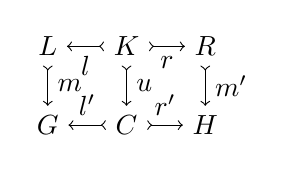
\begin{tikzpicture}
            % [node distance=15mm]
            \node (I) {$K$};
            \node (L) [left of=I] {$L$};
            \node (R) [right of=I] {$R$};
            \node (G) [below of=L] {$G$};
            \node (C) [below of=I] {$C$};
            \node (H) [below of=R] {$H$}; 
            \draw [>->] (I) to  node [midway,below] {$l$} (L);
            \draw [>->] (I) to  node [midway,below] {$r$} (R);
            \draw [>->] (L) to node [midway,right] {$m$} (G);
            \draw [>->] (I) to  node [midway,right] {$u$} (C); 
            \draw [>->] (R) to  node [midway,right] {$m'$} (H);
            \draw [>->] (C) to node [midway,above] {$l'$} (G);
            \draw [>->] (C) to node [midway,above] {$r'$} (H);
            % \node [at=($(I)!.5!(G)$)] {\normalfont PO};
            % \node [at=($(I)!.5!(H)$)] {\normalfont PO};
        \end{tikzpicture}
    \end{minipage} 

   $$
        \card{\operatorname{Mono}(\mathcal{X},G,\lnot m, l')_{\operatorname{NF}}} \geq
        \card{\operatorname{Mono}(\mathcal{X},H,\lnot m', r')_{\operatorname{NF}}}$$
\end*{}
\begin{proof}
    \label{antipattern:proof:lem:xglnotmlp_xhlnotmrp}
    There are two cases to consider: either $\mathcal{X} = (X)$ or $\mathcal{X} = (X, f:X \rightarrowtail F)$. 
     In the first case, since there is no forbidden context, the inequality is equivalent to $
        \card{\operatorname{Mono}(\mathcal{X},G,\lnot m, l')} \geq
        \card{\operatorname{Mono}(\mathcal{X},H,\lnot m', r')}$.
    To show this inequality, we are going to establish an injection from $\operatorname{Mono}(\mathcal{X},H,\lnot m', r')$ to $\operatorname{Mono}(\mathcal{X},G,\lnot m, l')$. Let $h_{XH} \in \operatorname{Mono}(\mathcal{X},H,\lnot m', r')$. By definition, there exists a monomorphism $h_{XC}:X \rightarrowtail C$ such that $h_{XH} = h_{XC} \star r'$. Thus we have the following commutative diagram:

     \begin{center}
    \begin{tikzpicture}
        \node (k) at (0,1) {K};
        \node (l) at (-2,1) {L};
        \node (r) at (2,1) {R};
        \node (c) at (0,-1) {C};
        \node (g) at (-2,-1) {G};
        \node (h) at (2,-1) {H};
        \node (x) at (4,-2) {X};
        \draw[>->] (x) -- (h) node [midway,above] {};
        \draw[>->] (x) edge (c) node [midway,above] {};
        \draw[>->]  (k) -- (r) node [midway,below] {r};
        \draw[>->]  (k) -- (l) node [midway,below] {l};
        \draw[>->] (c) -- (g) node [midway, above] {l'};
        \draw[>->] (c) -- (h) node [midway,above] {r'};
        \draw[>->] (l) -- (g) node[midway, right] {m};
        \draw[>->] (r) -- (h) node[midway, left] {m'};
        \draw[>->] (k) -- (c) node[midway, left] {u};
        \node () [at=($(l)!0.5!(c)$)] {PO};
        \node () [at=($(r)!0.5!(c)$)] {PO};
    \end{tikzpicture}
    \end{center}
    We must show $h_{XC} \star l' \in \operatorname{Mono}(\mathcal{X},G,\lnot m, l')$ which is equivalent to showing that there is no $h_{XL}$ such that 
    $h_{XL} \star m = h_{XC} \star l'$.
    Suppose that the contrary holds.
     Since $KLGC$ is a pullback by~\autoref{prop:pb_eq_po}, there is a morphism $h_{XK}:X \rightarrowtail K$ such that 
            \begin{flalign}
         h_{XK} \star u = h_{XC} \label{alabeldkfsjlk}
        \end{flalign} Therefore, we have 
    \begin{flalign*}
        h_{XH} 
        &= h_{XC} \star r' \\
        &= (h_{XK} \star u) \star r' \hspace{1cm} by~\eqref{alabeldkfsjlk}\\
        &= h_{XK} \star (r \star m') \\ 
        &= (h_{XK} \star r) \star m' 
    \end{flalign*}
    which contradicts the fact that $h_{XH} \in \operatorname{Mono}(\mathcal{X},H,\lnot m', r')$. Therefore, we have $h_{XC} \star l' \in \operatorname{Mono}(\mathcal{X},G,\lnot m, l')$.

    Furthermore, if $h_{XH}, h_{XH}' \in \operatorname{Mono}(\mathcal{X},H,\lnot m', r')$ with $h_{XH} \neq h_{XH}'$, then there exist $h_{XC}, h_{XC}'$ such that $h_{XH} = h_{XC} \star r'$ and $h_{XH}' = h_{XC}' \star r'$. Since $r'$ is injective, we deduce that $h_{XC} \neq h_{XC}'$. Therefore, from the injectivity of $l'$, we have $h_{XC} \star l' \neq h_{XC}' \star l'$. Thus, there is an injection from $\operatorname{Mono}(\mathcal{X},H,\lnot m', r')$ to $\operatorname{Mono}(\mathcal{X},G,\lnot m, l')$, which proves the inequality.
        
        Now, let us focus on the second case, where $\mathcal{X} = (X, f:X \rightarrowtail F)$. We have the following equalities:
        \begin{flalign*}
            &\card{\operatorname{Mono}(\mathcal{X},G,\lnot m, l')_{\operatorname{NF}}} - 
            \card{\operatorname{Mono}(,H,\lnot m', r')_{\operatorname{NF}}} 
           \\
            = &(\card{\operatorname{Mono}(X,G,\lnot m, l')} - \card{\operatorname{Mono}(\mathcal{X},G,\lnot m, l')_{\operatorname{F}}}) - \\
              &(\card{\operatorname{Mono}(X,H,\lnot m', r')} - \card{\operatorname{Mono}(\mathcal{X},H,\lnot m', r')_{\operatorname{F}}})
            \\
            = &(\card{\operatorname{Mono}(X,G,\lnot m, l')} - \card{\operatorname{Mono}(X,H,\lnot m', r')}) +\\ 
              &(\card{\operatorname{Mono}(\mathcal{X},H,\lnot m', r')_{\operatorname{F}}} - \card{\operatorname{Mono}(\mathcal{X},G,\lnot m, l')_{\operatorname{F}}})
               \\
            = & (\card{\operatorname{Mono}(X,C,\lnot u)} - \card{\operatorname{Mono}(X,C,\lnot u)}) + \\
              & (\card{\operatorname{Mono}(\mathcal{X},H,\lnot m', r')_{\operatorname{F}}} - \card{\operatorname{Mono}(\mathcal{X},G,\lnot m, l')_{\operatorname{F}}})
            \\
            &\text{By~\autoref{subgraph_counting:lem:decomp_w_u}}
            \\
            = & \card{\operatorname{Mono}(\mathcal{X},H,\lnot m', r')_{\operatorname{F}}} - \card{\operatorname{Mono}(\mathcal{X},G,\lnot m, l')_{\operatorname{F}}}
        \end{flalign*}
    We prove this lemma by show that the function $\phi:\operatorname{Mono}(\mathcal{X},G,\lnot m, l')_{\operatorname{F}} \rightarrow \operatorname{Mono}(\mathcal{X},H,\lnot m', r')_{\operatorname{NF}}$
    defined by $\phi(h_{XG}) = h_{XC} \star r'$ for all $h_{XG} \in \operatorname{Mono}(\mathcal{X},G,\lnot m, l')_{\operatorname{F}}$, where $h_{XC}:X \rightarrowtail C$ is the uniquemonomorphism such that $h_{XG} = h_{XC} \star l'$, is injective.

    We first show that $\phi$ is well-defined.

    Let $h_{XG} \in \operatorname{Mono}(\mathcal{X},G,\lnot m, l')_{\operatorname{F}}$. By definition, there are $h_{FG}:F \rightarrowtail G$ and $h_{XC}:X \rightarrowtail C$ such that
        \begin{flalign}
            h_{XG} &= h_{XC} \star l' \label{antipattern:lem:hxghxclp} \\
            h_{XF} \star h_{FG} &= H_{XG} \label{antipattern:lem:hxfhfghxg}
        \end{flalign}
    Therefore, the following commutative diagram holds:

    \begin{center}
    \begin{tikzpicture}
        \node (k) at (0,1) {K};
        \node (l) at (-2,1) {L};
        \node (r) at (2,1) {R};
        \node (c) at (0,-1) {C};
        \node (g) at (-2,-1) {G};
        \node (h) at (2,-1) {H};
        \node (x) at (-4,-1) {X};
        \node (f) at  (-4,-2) {F};
        \draw[>->] (x) -- (g) node [midway,above] {};
        \draw[>->] (x) -- (f) node [midway,above] {};
        \draw[>->]  (f) -- (g) node [midway,above] {};
        % \draw[>->] (x) -- (l) node [midway,above] {};
        \draw[>->] (x) edge [bend right](c) node [midway,above] {};
        \draw[>->]  (k) -- (r) node [midway,below] {r};
        \draw[>->]  (k) -- (l) node [midway,below] {l};
        \draw[>->] (c) -- (g) node [midway, above] {l'};
        \draw[>->] (c) -- (h) node [midway,above] {r'};
        \draw[>->] (l) -- (g) node[midway, right] {m};
        \draw[>->] (r) -- (h) node[midway, left] {m'};
        \draw[>->] (k) -- (c) node[midway, left] {u};
        \node () [at=($(l)!0.5!(c)$)] {PO};
        \node () [at=($(r)!0.5!(c)$)] {PO};
    \end{tikzpicture}
    \end{center}


   We prove that $\phi(h_{XG})$ cannot be factorized by $m'$, by contradiction. Suppose that the contrary holds, i.e. there is $h_{XR}:X \rightarrow R$ such that $\phi(h_{XG}) \overset{def}{=} h_{XC} \star r' = h_{XR} \star m'$. The morphism $h_{XR}$ is injective, because $\phi(h_{XG})$ is injective. Therefore, under this assumption, we have the following commutative diagram:

    \begin{tikzpicture}
       \node (k) at (0,1) {K};
       \node (l) at (-2,1) {L};
       \node (r) at (2,1) {R};
       \node (c) at (0,-1) {C};
       \node (g) at (-2,-1) {G};
       \node (h) at (2,-1) {H};
       \node (x) at (-4,-1) {X};
       \node (f) at  (-4,-2) {F};
       \draw[>->] (x) -- (g) node [midway,above] {};
       \draw[>->] (x) -- (f) node [midway,above] {};
       \draw[>->]  (f) -- (g) node [midway,above] {};
       % \draw[>->] (x) -- (l) node [midway,above] {};
       \draw[>->] (x) edge [bend right](c) node [midway,above] {};
       \draw[>->] (x) edge [out=90,in=135](r) node [midway,above] {};
       \draw[>->] (f) edge [bend right](c) node [midway,above] {};
       \draw[>->]  (k) -- (r) node [midway,below] {r};
       \draw[>->]  (k) -- (l) node [midway,below] {l};
       \draw[>->] (c) -- (g) node [midway, above] {l'};
       \draw[>->] (c) -- (h) node [midway,above] {r'};
       \draw[>->] (l) -- (g) node[midway, right] {m};
       \draw[>->] (r) -- (h) node[midway, left] {m'};
       \draw[>->] (k) -- (c) node[midway, left] {u};
       \node () [at=($(l)!0.5!(c)$)] {PO};
       \node () [at=($(r)!0.5!(c)$)] {PO};
   \end{tikzpicture}
   
   \noindent
    The square $KCHR$ is also a pullback by~\autoref{prop:pb_eq_po}. 
    By the universal property of pullback, there exists a unique morphism $h_{XK}:X \rightarrow K$, which is injective because $h_{XR}$ is injective, such that $h_{XK} \star r = h_{XR}$ and 
    \begin{flalign}
        h_{XK} \star u = h_{XC} \label{antipattern:eq:hxk_u}
    \end{flalign} 
    Therefore, the following commutative diagram holds:

%      \begin{tikzpicture}
%        \node (k) at (0,1) {K};
%        \node (l) at (-2,1) {L};
%        \node (r) at (2,1) {R};
%        \node (c) at (0,-1) {C};
%        \node (g) at (-2,-1) {G};
%        \node (h) at (2,-1) {H};
%        \node (x) at (-4,2) {X};
%        \node (f) at  (-4,-2) {F};
%        \draw[>->] (x) -- (g) node [midway,above] {};
%        \draw[>->] (x) -- (f) node [midway,above] {};
%        \draw[>->]  (f) -- (g) node [midway,above] {};
%        % \draw[>->] (x) -- (l) node [midway,above] {};
%        \draw[>->] (x) edge[out=-80,in=220] (c) node [midway,above] {};
%        \draw[>->] (x) edge
%         % [out=90,in=135]
%         (r) node [midway,above] {};
%        \draw[>->] (f) edge [out=0,in=-90](c) node [midway,above] {};
%        \draw[>->]  (k) -- (r) node [midway,below] {r};
%        \draw[>->]  (k) -- (l) node [midway,below] {l};
%        \draw[>->] (c) -- (g) node [midway, above] {l'};
%        \draw[>->] (c) -- (h) node [midway,above] {r'};
%        \draw[>->] (l) -- (g) node[midway, right] {m};
%        \draw[>->] (x) -- (k) node[midway, right] {};
%        \draw[>->] (r) -- (h) node[midway, left] {m'};
%        \draw[>->] (k) -- (c) node[midway, left] {u};
%        \node () [at=($(l)!0.5!(c)$)] {PO};
%        \node () [at=($(r)!0.5!(c)$)] {PB};
%    \end{tikzpicture}
       \begin{tikzpicture}
       \node (k) at (0,1) {K};
       \node (l) at (-2,1) {L};
       \node (r) at (2,1) {R};
       \node (c) at (0,-1) {C};
       \node (g) at (-2,-1) {G};
       \node (h) at (2,-1) {H};
       \node (x) at (-4,-1) {X};
       \node (f) at  (-4,-2) {F};
       \draw[>->] (x) -- (g) node [midway,above] {};
       \draw[>->] (x) -- (f) node [midway,above] {};
       \draw[>->]  (f) -- (g) node [midway,above] {};
       % \draw[>->] (x) -- (l) node [midway,above] {};
       \draw[>->] (x) edge [bend right](c) node [midway,above] {};
       \draw[>->] (x) edge [out=90,in=135](r) node [midway,above] {};
       \draw[>->] (x) edge [out=90,in=135](k) node [midway,above] {};
       \draw[>->] (f) edge [bend right](c) node [midway,above] {};
       \draw[>->]  (k) -- (r) node [midway,below] {r};
       \draw[>->]  (k) -- (l) node [midway,below] {l};
       \draw[>->] (c) -- (g) node [midway, above] {l'};
       \draw[>->] (c) -- (h) node [midway,above] {r'};
       \draw[>->] (l) -- (g) node[midway, right] {m};
       \draw[>->] (r) -- (h) node[midway, left] {m'};
       \draw[>->] (k) -- (c) node[midway, left] {u};
       \node () [at=($(l)!0.5!(c)$)] {PO};
       \node () [at=($(r)!0.5!(c)$)] {PB};
   \end{tikzpicture}
   
   \noindent 
   Thus, we have \begin{flalign*}
        h_{XG} &= h_{XC} \star l' \\
        &= (h_{XK} \star u) \star l' &\text{by~\eqref{antipattern:eq:hxk_u}}\\
        &= h_{XK} \star (l \star m)  &\text{by commutativity of $KLGC$}
    \end{flalign*}
    Which is a contradiction because $h_{XG}$ is an element of $\operatorname{Mono}(\mathcal{X},G,\lnot m, l')_{\operatorname{F}}$ and, by definition, cannot be factorized by $m$. Thus, the assumption is false, and $\phi(h_{XG})$ cannot be factorized by $m'$.

    % In order to show that $\phi(h_{XG})$ is an element in $\operatorname{Mono}(\mathcal{X},H,\lnot m', r')_{\operatorname{F}}$, since $\phi(h_{XG})$ can be factorized by $r'$ by definition, 
    Consider the commutative diagram shown below.
    It remains to show that $\phi(h_{XG})$ can be decomposed as $x \star y$ with $x: X \rightarrowtail F$ and $y: F \rightarrowtail H$. There are three mutually exclusive cases according to whether or not the morphism $h_{FG}$ can be factorized by $m$ or $l'$.
        \begin{center}
    \begin{tikzpicture}
        \node (k) at (0,1) {K};
        \node (l) at (-2,1) {L};
        \node (r) at (2,1) {R};
        \node (c) at (0,-1) {C};
        \node (g) at (-2,-1) {G};
        \node (h) at (2,-1) {H};
        \node (x) at (-4,-1) {X};
        \node (f) at  (-4,-2) {F};
        \draw[>->] (x) -- (g) node [midway,above] {};
        \draw[>->] (x) -- (f) node [midway,above] {};
        \draw[>->]  (f) -- (g) node [midway,above] {};
        % \draw[>->] (x) -- (l) node [midway,above] {};
        \draw[>->] (x) edge [bend right](c) node [midway,above] {};
        \draw[>->]  (k) -- (r) node [midway,below] {r};
        \draw[>->]  (k) -- (l) node [midway,below] {l};
        \draw[>->] (c) -- (g) node [midway, above] {l'};
        \draw[>->] (c) -- (h) node [midway,above] {r'};
        \draw[>->] (l) -- (g) node[midway, right] {m};
        \draw[>->] (r) -- (h) node[midway, left] {m'};
        \draw[>->] (k) -- (c) node[midway, left] {u};
        \node () [at=($(l)!0.5!(c)$)] {PO};
        \node () [at=($(r)!0.5!(c)$)] {PO};
    \end{tikzpicture}
    \end{center}
    %  $h_{FG}$ can be factorized by $m$ or $l'$:
    \begin{itemize}
        \item Case 1 : there exists $h_{FL}: F \rightarrow L$ such that $h_{FG} = h_{FL} \star m$. 
        This case is impossible, because if it were true, then we would have the following commutative diagram:

        \begin{tikzpicture}
            \node (k) at (0,1) {K};
            \node (l) at (-2,1) {L};
            \node (r) at (2,1) {R};
            \node (c) at (0,-1) {C};
            \node (g) at (-2,-1) {G};
            \node (h) at (2,-1) {H};
            \node (x) at (-4,-1) {X};
            \node (f) at  (-4,-2) {F};
            \draw[>->] (x) -- (g) node [midway,above] {};
            \draw[>->] (x) -- (f) node [midway,above] {};
            \draw[>->]  (f) -- (g) node [midway,above] {};
            \draw[>->] (f) -- (l) node [midway,above] {};
            \draw[>->] (x) edge [bend right](c) node [midway,above] {};
            \draw[>->]  (k) -- (r) node [midway,below] {r};
            \draw[>->]  (k) -- (l) node [midway,below] {l};
            \draw[>->] (c) -- (g) node [midway, above] {l'};
            \draw[>->] (c) -- (h) node [midway,above] {r'};
            \draw[>->] (l) -- (g) node[midway, right] {m};
            \draw[>->] (r) -- (h) node[midway, left] {m'};
            \draw[>->] (k) -- (c) node[midway, left] {u};
            \node () [at=($(l)!0.5!(c)$)] {PO};
            \node () [at=($(r)!0.5!(c)$)] {PO};
        \end{tikzpicture}
        
        Therefore, we would have 
        \begin{flalign*}
             h_{XC} \star l' = &h_{XG}  & \text{by~\eqref{antipattern:lem:hxghxclp}}\\
             = &f \star h_{FG} 
             &\text{by~\eqref{antipattern:lem:hxfhfghxg}} \\
             = &f \star h_{FL} \star m \\
        \end{flalign*} which would imply that $h_{XC}$ is not in $\operatorname{Mono}(X,G,\lnot m, l')$.
        \item Case 2 : there does not exist $h_{FL}: F \rightarrow L$ such that $h_{FG} = h_{FL} \star m$, but there exists $h_{FC}:F \rightarrow C$ such that $h_{FG} = h_{FC} \star l'$. 
        We have the following commutative diagram:

        \begin{tikzpicture}
            \node (k) at (0,1) {K};
            \node (l) at (-2,1) {L};
            \node (r) at (2,1) {R};
            \node (c) at (0,-1) {C};
            \node (g) at (-2,-1) {G};
            \node (h) at (2,-1) {H};
            \node (x) at (-4,-1) {X};
            \node (f) at  (-4,-2) {F};
            \draw[>->] (x) -- (g) node [midway,above] {};
            \draw[>->] (x) -- (f) node [midway,above] {};
            \draw[>->]  (f) -- (g) node [midway,above] {};
            % \draw[>->] (x) -- (l) node [midway,above] {};
            \draw[>->] (x) edge [bend right](c) node [midway,above] {};
            \draw[>->] (f) edge [bend right](c) node [midway,above] {};
            \draw[>->]  (k) -- (r) node [midway,below] {r};
            \draw[>->]  (k) -- (l) node [midway,below] {l};
            \draw[>->] (c) -- (g) node [midway, above] {l'};
            \draw[>->] (c) -- (h) node [midway,above] {r'};
            \draw[>->] (l) -- (g) node[midway, right] {m};
            \draw[>->] (r) -- (h) node[midway, left] {m'};
            \draw[>->] (k) -- (c) node[midway, left] {};
            \node () [at=($(l)!0.5!(c)$)] {PO};
            \node () [at=($(r)!0.5!(c)$)] {PO};
        \end{tikzpicture}

        We have therefore $\phi(h_{XG}) = h_{XC} \star r' = h_{XF} \star (h_{FC} \star r')$.

    \item Case 3 : there does not exist $h_{FL}: F \rightarrow L$ such that $h_{FG} = h_{FL} \star m$,
    and there does not exist $h_{FC}:F \rightarrow C$ such that $h_{FG} = h_{FC} \star l'$.
     By~\autoref{antipattern:lem:xh_decomp}, we can construct the following commutative diagram:

    \begin{center}
        \resizebox{0.3\textwidth}{!}{
            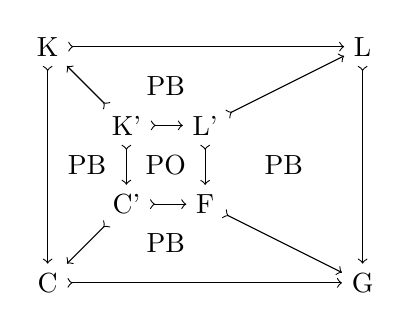
\begin{tikzpicture}
                \node (k) at (0,0) {K};
                \node (r) at (4,0) {L};
                \node (c) at (0,-3) {C};
                \node (h) at (4,-3) {G};
                \draw[<-<]  (r) -- (k) node [midway,above] {};
                \draw[>->] (c) -- (h) node [midway, below] {};
                \draw[>->] (r) -- (h) node[midway, left] {};
                \draw[>->] (k) -- (c) node[midway, left] {};
                \node (k') at (1,-1) {K'};
                \node (r') at (2,-1) {L'};
                \node (c') at (1,-2) {C'};
                \node () at (1.5,-1.5) {PO};
                \node () at (3,-1.5) {PB};
                \node () at (1.5,-2.5) {PB};
                \node () at (1.5,-0.5) {PB};
                \node () at (0.5,-1.5) {PB};
                \node (x) at (2,-2) {F};
                \draw [>->] (c') -- (x);
                \draw [>->] (r') -- (x);
                \draw [>->] (k') -- (r');
                \draw [>->] (k') -- (c');
                \draw [>->] (c') -- (c);
                \draw[>->] (r') -- (r);
                \draw[>->] (x) -- (h) node[midway,right] {};
                \draw[>->] (k') -- (k) ;
            \end{tikzpicture}
        }
        \end{center} 

    There exists a unique monomorphism $h_{XC'}:X \rightarrowtail C'$ 
    such that $h_{XC'} \star h_{C'C} = h_{XC}$ and $h_{XC'} \star h_{C'F} = h_{XF}$,
    because we have $h_{XF} \star h_{FG} = h_{XG}$, $h_{XC} \star h_{CG} = h_{XG}$ and $C'CGF$ is a pullback.


    Thus, we have the following commutative diagram:
    \begin{center}
        \resizebox{0.3\textwidth}{!}{
            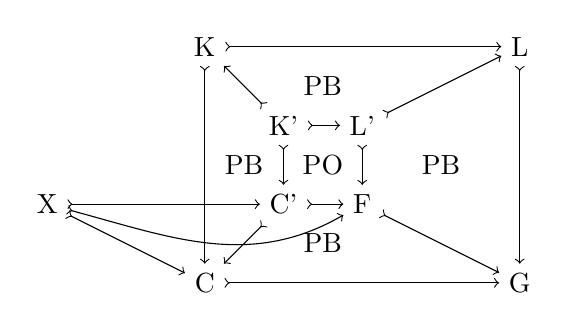
\begin{tikzpicture}
                \node (k) at (0,0) {K};
                \node (r) at (4,0) {L};
                \node (c) at (0,-3) {C};
                \node (h) at (4,-3) {G};
                % \node (rb) at ($\scl*(1.5,-0.5)$) {$R_X$};
                % \node (h') at ($\scl*(1.5,-1.5)$) {$H'$};
                % \draw[>->]  (rb) -- (h') node [midway,above] {};
                % \draw[>->]  (c) -- (h') node [midway,above] {};
                \draw[<-<]  (r) -- (k) node [midway,above] {};
                \draw[>->] (c) -- (h) node [midway, below] {$$};
                \draw[>->] (r) -- (h) node[midway, left] {$$};
                \draw[>->] (k) -- (c) node[midway, left] {};
                % \draw[->] (rb) to (l);
                % \draw[<-<] (rb) to (k);
                \node (k') at (1,-1) {K'};
                \node (r') at (2,-1) {L'};
                \node (x') at (-2,-2) {X};
                \node (c') at (1,-2) {C'};
                \node () at (1.5,-1.5) {PO};
                \node () at (3,-1.5) {PB};
                \node () at (1.5,-2.5) {PB};
                \node () at (1.5,-0.5) {PB};
                \node () at (0.5,-1.5) {PB};
                \node (x) at (2,-2) {F};
                % \draw [->] (x) -- (h') node[midway] {!};
                \draw [>->] (c') -- (x);
                \draw [>->] (x') -- (c');
                \draw [>->] (x') -- (c);
                \draw [>->] (x') edge[out=-15,in=210] (x);
                \draw [>->] (r') -- (x);
                \draw [>->] (k') -- (r');
                \draw [>->] (k') -- (c');
                \draw [>->] (c') -- (c);
                % \draw [->] (r') -- (rb);
                % \draw [->] (r') -- (rb);
                % \draw [->] (h') -- (h);
                \draw[>->] (r') -- (r) node[midway,below] {};
                \draw[>->] (x) -- (h) node[midway,right] {};
                % \node (rb) at ($\scl*(\sclx*1.5,-0.5)$) {$R_X$};
                % \node (h') at ($\scl*(\sclx*1.5,-1.2)$) {$H'$};
                % \draw[>->]  (rb) -- (h') node [midway,above] {};
                % \draw[>->]  (c) -- (h') node [midway,above] {};
                % \draw[>->]  (rb) -- (h') node [midway,above] {};
                % \draw[>->] (rb) to (r);
                % \draw[<-<] (rb) to (k);
                \draw[>->] (k') -- (k) ;
            \end{tikzpicture}
        }
        \end{center} 
    
     By the $F$-non-increasing property of $\rho^{-1}$,  
     \todo{assumption: the $F$-non-increasing property of $\rho^{-1}$}$h_{L'R}$ 
     there is a morphism $h_{L'R}:L' \rightarrowtail R$ such that $K'L'RK$ is a pullback.
        By~\autoref{lem:g_monic}, there exists a unique monomorphism $h_{FH}:F \rightarrowtail H$ such that $L'FHR$ and $C'FHC$ are commutative squares.
    %      $h_{L'R} \star h_{RH} = h_{L'F} \star h_{FH}$ and $h_{C'F} \star h_{FH} = h_{C'C} \star h_{CH}$, because $K'C'FL'$ is a pushout, and 
    % \begin{flalign*}
    %      &h_{K'L'} \star h_{L'R} \star h_{RH} \\
    %     =&h_{K'K} \star h_{KR} \star h_{RH} \\
    %     =&h_{K'K} \star h_{KC} \star h_{CH} \\
    %     =&h_{K'C'} \star h_{C'C} \star h_{CH}
    % \end{flalign*} 

    Thus, we have the following commutative diagram:
    \begin{center}
        \resizebox{0.3\textwidth}{!}{
            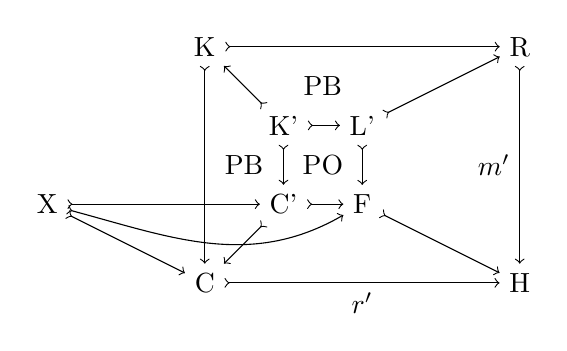
\begin{tikzpicture}
                \node (k) at (0,0) {K};
                \node (r) at (4,0) {R};
                \node (c) at (0,-3) {C};
                \node (h) at (4,-3) {H};
                % \node (rb) at ($\scl*(1.5,-0.5)$) {$R_X$};
                % \node (h') at ($\scl*(1.5,-1.5)$) {$H'$};
                % \draw[>->]  (rb) -- (h') node [midway,above] {};
                % \draw[>->]  (c) -- (h') node [midway,above] {};
                \draw[<-<]  (r) -- (k) node [midway,above] {};
                \draw[>->] (c) -- (h) node [midway, below] {$r'$};
                \draw[>->] (r) -- (h) node[midway, left] {$m'$};
                \draw[>->] (k) -- (c) node[midway, left] {};
                % \draw[->] (rb) to (l);
                % \draw[<-<] (rb) to (k);
                \node (k') at (1,-1) {K'};
                \node (r') at (2,-1) {L'};
                \node (x') at (-2,-2) {X};
                \node (c') at (1,-2) {C'};
                \node () at (1.5,-1.5) {PO};
                % \node () at (3,-1.5) {PB};
                % \node () at (1.5,-2.5) {PB};
                \node () at (1.5,-0.5) {PB};
                \node () at (0.5,-1.5) {PB};
                \node (x) at (2,-2) {F};
                % \draw [->] (x) -- (h') node[midway] {!};
                \draw [>->] (c') -- (x);
                \draw [>->] (x') -- (c');
                \draw [>->] (x') -- (c);
                \draw [>->] (x') edge[out=-15,in=210] (x);
                \draw [>->] (r') -- (x);
                \draw [>->] (k') -- (r');
                \draw [>->] (k') -- (c');
                \draw [>->] (c') -- (c);
                % \draw [->] (r') -- (rb);
                % \draw [->] (r') -- (rb);
                % \draw [->] (h') -- (h);
                \draw[>->] (r') -- (r) node[midway,below] {};
                \draw[>->] (x) -- (h) node[midway,right] {};
                % \node (rb) at ($\scl*(\sclx*1.5,-0.5)$) {$R_X$};
                % \node (h') at ($\scl*(\sclx*1.5,-1.2)$) {$H'$};
                % \draw[>->]  (rb) -- (h') node [midway,above] {};
                % \draw[>->]  (c) -- (h') node [midway,above] {};
                % \draw[>->]  (rb) -- (h') node [midway,above] {};
                % \draw[>->] (rb) to (r);
                % \draw[<-<] (rb) to (k);
                \draw[>->] (k') -- (k) ;
            \end{tikzpicture}
        }
        \end{center} 

        Finally, we have:
        \begin{flalign*}
            \phi(h_{XG}) &= h_{XC} \star r' \\
            &= h_{XC'} \star h_{C'C} \star r' \\
            &= (h_{XC'} \star h_{C'F}) \star h_{FH}  \\
        \end{flalign*} 
    \end{itemize}
    We have thus shown that $\phi$ is well defined.
    
    Proving its injectivity is straightforward. 
    Let $h_{XG}, h_{XG}' \in \operatorname{Mono}(\mathcal{X},G,\lnot m, l')_{\operatorname{F}}$ such that $h_{XG} \neq h_{XG}'$.
    There exist $h_{XC},h_{XC}'$ such that $h_{XG} = h_{XC} \star l'$ and $h_{XG}' = h_{XC}' \star l'$.
    By injectivity of $l'$, we have $h_{XC} \neq h_{XC}'$. Therefore, we have $\phi(h_{XG}) = h_{XC} \star r' \neq h_{XC}' \star r' = \phi(h_{XG}')$ because $r'$ is injective.
\end{proof} 

\noindent
\begin*{\textbf{\autoref{lem:xglnotmlnotlp_xhlnotmrnotrp}}}
    \newline
    \noindent
    \vspace{2mm}
    \begin{minipage}{0.7\textwidth}\setlength{\parindent}{1em}
        Let $\mathcal{X}$ be a ruler-graph with underlying graph $X$, and let \( \rho = (L \overset{l}{\leftarrowtail} K \overset{r}{\rightarrowtail} R) \) be a rule. Suppose that $\rho$ and $\rho^{-1}$ are $X$-non-increasing.
        Consider the DPO diagram illustrated on the right. We have 
    \end{minipage}%
    \begin{minipage}{0.29\textwidth}
        \hfill
        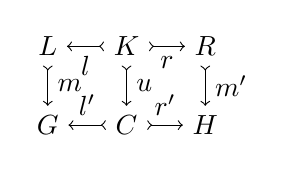
\begin{tikzpicture}
            % [node distance=15mm]
            \node (I) {$K$};
            \node (L) [left of=I] {$L$};
            \node (R) [right of=I] {$R$};
            \node (G) [below of=L] {$G$};
            \node (C) [below of=I] {$C$};
            \node (H) [below of=R] {$H$}; 
            \draw [>->] (I) to  node [midway,below] {$l$} (L);
            \draw [>->] (I) to  node [midway,below] {$r$} (R);
            \draw [>->] (L) to node [midway,right] {$m$} (G);
            \draw [>->] (I) to  node [midway,right] {$u$} (C); 
            \draw [>->] (R) to  node [midway,right] {$m'$} (H);
            \draw [>->] (C) to node [midway,above] {$l'$} (G);
            \draw [>->] (C) to node [midway,above] {$r'$} (H);
            % \node [at=($(I)!.5!(G)$)] {\normalfont PO};
            % \node [at=($(I)!.5!(H)$)] {\normalfont PO};
        \end{tikzpicture}
    \end{minipage} 
    $$
        \card{\operatorname{Mono}(\mathcal{X},G,\lnot m, \lnot l')_{\operatorname{NF}}} \geq
        \card{\operatorname{Mono}(\mathcal{X},H,\lnot m', \lnot r')_{\operatorname{NF}}}
    $$
\end*{}
\begin{proof} 
      \label{antipattern:proof:lem:xglnotmlnotlp_xhlnotmrnotrp}
    There are two cases to consider: the ruler-graph is $(X)$ or $(X,f:X \rightarrowtail F)$. For the first case, the inequality is equivalent to 
 $
        \card{\operatorname{Mono}(\mathcal{X},G,\lnot m, \lnot l')} \geq
        \card{\operatorname{Mono}(\mathcal{X},H,\lnot m', \lnot r')}
    $
    , and the result follows from~\autoref{subgraph_counting:lem:w_u_l_not_geq_r_not}. 
    Let us now consider the second case.
     \todo{assumption for~\autoref{subgraph_counting:lem:w_u_l_not_geq_r_not}: $\rho$ is $X$-non-increasing} The following equalities and inequalities hold:
    \begin{flalign*}
        & \card{\operatorname{Mono}(\mathcal{X},G,\lnot m, \lnot l')_{\operatorname{NF}}} - 
        \card{\operatorname{Mono}(\mathcal{X},H,\lnot m', \lnot r')_{\operatorname{NF}}} 
        \\
        = &(\card{\operatorname{Mono}(X,G,\lnot m, \lnot l')} - \card{\operatorname{Mono}(\mathcal{X},G,\lnot m, \lnot l')_{\operatorname{F}}}) -
            \\ 
           &(\card{\operatorname{Mono}(X,H,\lnot m', \lnot r')} - \card{\operatorname{Mono}(\mathcal{X},H,\lnot m', \lnot r')_{\operatorname{F}}})
        \\
        = &(\card{\operatorname{Mono}(X,G,\lnot m, \lnot l')} - \card{\operatorname{Mono}(X,H,\lnot m', \lnot r')}) + 
        \\ 
        &
           (\card{\operatorname{Mono}(\mathcal{X},H,\lnot m', \lnot r')_{\operatorname{F}}} - 
           \card{\operatorname{Mono}(\mathcal{X},G,\lnot m, \lnot l')_{\operatorname{F}}})
           \\
        \geq & 
            \card{\operatorname{Mono}(\mathcal{X},H,\lnot m', \lnot r')_{\operatorname{F}}} 
            - 
            \card{\operatorname{Mono}(\mathcal{X},G,\lnot m, \lnot l')_{\operatorname{F}}}
        \\
        & \text{by~\autoref{subgraph_counting:lem:w_u_l_not_geq_r_not}}
    \end{flalign*}    

    % We prove this lemma by show that the function $\phi: \operatorname{Mono}(\mathcal{X},G,\lnot m, \lnot l')_{\operatorname{F}} \rightarrowtail \operatorname{Mono}(X,H,\lnot r', \lnot r')_{\operatorname{NF}}$
    % defined by $\phi(h_{XG}) = h_{XC} \star \lnot r'$ is injective where $h_{XC}:X \rightarrowtail C$ is a monomorphism such that $h_{XG} = h_{XC} \star \lnot l'$.

    We prove $\card{\operatorname{Mono}(\mathcal{X},H,\lnot m', \lnot r')_{\operatorname{F}}} \geq \card{\operatorname{Mono}(\mathcal{X},G,\lnot m, \lnot l')_{\operatorname{F}}}$ by showing
    that we can construct an injection $\phi: \operatorname{Mono}(\mathcal{X},G,\lnot m, \lnot l')_{\operatorname{F}} \to \operatorname{Mono}(\mathcal{X},H,\lnot m', \lnot r')_{\operatorname{F}}$.

    Let $h_{XG} \in \operatorname{Mono}(\mathcal{X},G,\lnot m, \lnot l')_{\operatorname{F}}$. 
    By~\autoref{antipattern:lem:xh_decomp}, we can construct the following commutative diagram:

    \begin{center}
        \resizebox{0.3\textwidth}{!}{
            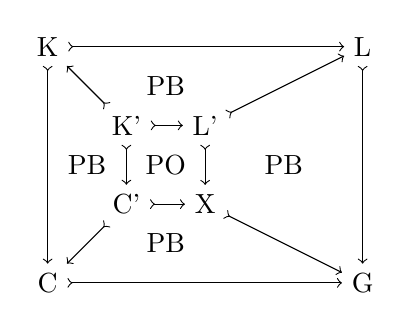
\begin{tikzpicture}
                \node (k) at (0,0) {K};
                \node (r) at (4,0) {L};
                \node (c) at (0,-3) {C};
                \node (h) at (4,-3) {G};
                % \node (rb) at ($\scl*(1.5,-0.5)$) {$R_X$};
                % \node (h') at ($\scl*(1.5,-1.5)$) {$H'$};
                % \draw[>->]  (rb) -- (h') node [midway,above] {};
                % \draw[>->]  (c) -- (h') node [midway,above] {};
                \draw[<-<]  (r) -- (k) node [midway,above] {};
                \draw[>->] (c) -- (h) node [midway, below] {};
                \draw[>->] (r) -- (h) node[midway, left] {};
                \draw[>->] (k) -- (c) node[midway, left] {};
                % \draw[->] (rb) to (l);
                % \draw[<-<] (rb) to (k);
                \node (k') at (1,-1) {K'};
                \node (r') at (2,-1) {L'};
                \node (c') at (1,-2) {C'};
                \node () at (1.5,-1.5) {PO};
                \node () at (3,-1.5) {PB};
                \node () at (1.5,-2.5) {PB};
                \node () at (1.5,-0.5) {PB};
                \node () at (0.5,-1.5) {PB};
                \node (x) at (2,-2) {X};
                % \draw [->] (x) -- (h') node[midway] {!};
                \draw [>->] (c') -- (x);
                \draw [>->] (r') -- (x);
                \draw [>->] (k') -- (r');
                \draw [>->] (k') -- (c');
                \draw [>->] (c') -- (c);
                % \draw [->] (r') -- (rb);
                % \draw [->] (r') -- (rb);
                % \draw [->] (h') -- (h);
                \draw[>->] (r') -- (r);
                \draw[>->] (x) -- (h) node[midway,right] {};
                % \node (rb) at ($\scl*(\sclx*1.5,-0.5)$) {$R_X$};
                % \node (h') at ($\scl*(\sclx*1.5,-1.2)$) {$H'$};
                % \draw[>->]  (rb) -- (h') node [midway,above] {};
                % \draw[>->]  (c) -- (h') node [midway,above] {};
                % \draw[>->]  (rb) -- (h') node [midway,above] {};
                % \draw[>->] (rb) to (r);
                % \draw[<-<] (rb) to (k);
                \draw[>->] (k') -- (k) ;
            \end{tikzpicture}
        }
        \end{center} 

         \todo{assmption: $\rho^{-1}$ is $X$-non-increasing} There exists a monomorphism $h_{L'R} : L' \rightarrowtail R$ because $\rho^{-1}$ is $X$-non-increasing by assumption. By~\autoref{lem:g_monic}, we can construct the following commutative diagram:

        \begin{center}
            \resizebox{0.3\textwidth}{!}{
                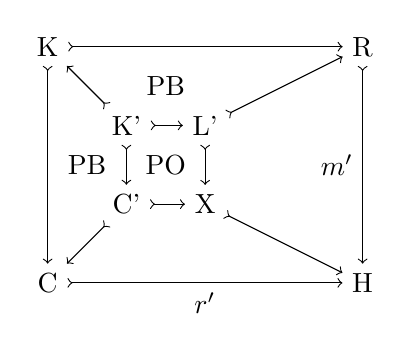
\begin{tikzpicture}
                    \node (k) at (0,0) {K};
                    \node (r) at (4,0) {R};
                    \node (c) at (0,-3) {C};
                    \node (h) at (4,-3) {H};
                    % \node (rb) at ($\scl*(1.5,-0.5)$) {$R_X$};
                    % \node (h') at ($\scl*(1.5,-1.5)$) {$H'$};
                    % \draw[>->]  (rb) -- (h') node [midway,above] {};
                    % \draw[>->]  (c) -- (h') node [midway,above] {};
                    \draw[<-<]  (r) -- (k) node [midway,above] {};
                    \draw[>->] (c) -- (h) node [midway, below] {$r'$};
                    \draw[>->] (r) -- (h) node[midway, left] {$m'$};
                    \draw[>->] (k) -- (c) node[midway, left] {};
                    % \draw[->] (rb) to (l);
                    % \draw[<-<] (rb) to (k);
                    \node (k') at (1,-1) {K'};
                    \node (r') at (2,-1) {L'};
                    \node (c') at (1,-2) {C'};
                    \node () at (1.5,-1.5) {PO};
                    % \node () at (3,-1.5) {PB};
                    % \node () at (1.5,-2.5) {PB};
                    \node () at (1.5,-0.5) {PB};
                    \node () at (0.5,-1.5) {PB};
                    \node (x) at (2,-2) {X};
                    % \draw [->] (x) -- (h') node[midway] {!};
                    \draw [>->] (c') -- (x);
                    \draw [>->] (r') -- (x);
                    \draw [>->] (k') -- (r');
                    \draw [>->] (k') -- (c');
                    \draw [>->] (c') -- (c);
                    % \draw [->] (r') -- (rb);
                    % \draw [->] (r') -- (rb);
                    % \draw [->] (h') -- (h);
                    \draw[>->] (r') -- (r) node[midway,below] {};
                    \draw[>->] (x) -- (h) node[midway,right] {};
                    % \node (rb) at ($\scl*(\sclx*1.5,-0.5)$) {$R_X$};
                    % \node (h') at ($\scl*(\sclx*1.5,-1.2)$) {$H'$};
                    % \draw[>->]  (rb) -- (h') node [midway,above] {};
                    % \draw[>->]  (c) -- (h') node [midway,above] {};
                    % \draw[>->]  (rb) -- (h') node [midway,above] {};
                    % \draw[>->] (rb) to (r);
                    % \draw[<-<] (rb) to (k);
                    \draw[>->] (k') -- (k) ;
                \end{tikzpicture}
            }
            \end{center} 

       
        We define $\phi(h_{XG}) \overset{def}{=} h_{XH}$. The function $\phi$ is injective, by~\autoref{lem:h_hp_diff_g_gp_diff} \todo{~\autoref{lem:h_hp_diff_g_gp_diff} uses the assumption: $\rho$ is $X$-non-increasing}. It remains to show that $\phi$ is well defined which requires to show that $\phi(h_{XG})$ is an element in $\operatorname{Mono}(X,H,\lnot m', \lnot r')_{\operatorname{F}}$, which is equivalent to show the following three conditions:
        \begin{enumerate}
            \item $h_{XH}$ cannot be factorized by $r'$,
            \item $h_{XH}$ cannot be factorized by $m'$,
            \item there is a monomorphism $h_{FH}:F \rightarrowtail H$ such that $h_{XH} = f \star h_{FH}$.
            % $h_{XH}$ can be decomposed as $x \star y$ where $x$ is a monomorphism from $X$ to $F$ and $y$ is a monomorphism from $F$ to $H$.
        \end{enumerate}

        By~\autoref{prop:graph_adhesive}, $KCHR$ is a VK-square. Therefore, we have the following commutative diagram:

        \begin{center}
            \resizebox{0.3\textwidth}{!}{
                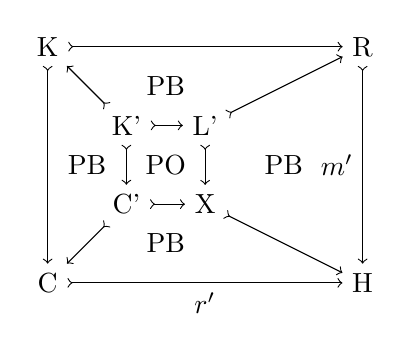
\begin{tikzpicture}
                    \node (k) at (0,0) {K};
                    \node (r) at (4,0) {R};
                    \node (c) at (0,-3) {C};
                    \node (h) at (4,-3) {H};
                    % \node (rb) at ($\scl*(1.5,-0.5)$) {$R_X$};
                    % \node (h') at ($\scl*(1.5,-1.5)$) {$H'$};
                    % \draw[>->]  (rb) -- (h') node [midway,above] {};
                    % \draw[>->]  (c) -- (h') node [midway,above] {};
                    \draw[<-<]  (r) -- (k) node [midway,above] {};
                    \draw[>->] (c) -- (h) node [midway, below] {$r'$};
                    \draw[>->] (r) -- (h) node[midway, left] {$m'$};
                    \draw[>->] (k) -- (c) node[midway, left] {};
                    % \draw[->] (rb) to (l);
                    % \draw[<-<] (rb) to (k);
                    \node (k') at (1,-1) {K'};
                    \node (r') at (2,-1) {L'};
                    \node (c') at (1,-2) {C'};
                    \node () at (1.5,-1.5) {PO};
                    \node () at (3,-1.5) {PB};
                    \node () at (1.5,-2.5) {PB};
                    \node () at (1.5,-0.5) {PB};
                    \node () at (0.5,-1.5) {PB};
                    \node (x) at (2,-2) {X};
                    % \draw [->] (x) -- (h') node[midway] {!};
                    \draw [>->] (c') -- (x);
                    \draw [>->] (r') -- (x);
                    \draw [>->] (k') -- (r');
                    \draw [>->] (k') -- (c');
                    \draw [>->] (c') -- (c);
                    % \draw [->] (r') -- (rb);
                    % \draw [->] (r') -- (rb);
                    % \draw [->] (h') -- (h);
                    \draw[>->] (r') -- (r) node[midway,below] {};
                    \draw[>->] (x) -- (h) node[midway,right] {};
                    % \node (rb) at ($\scl*(\sclx*1.5,-0.5)$) {$R_X$};
                    % \node (h') at ($\scl*(\sclx*1.5,-1.2)$) {$H'$};
                    % \draw[>->]  (rb) -- (h') node [midway,above] {};
                    % \draw[>->]  (c) -- (h') node [midway,above] {};
                    % \draw[>->]  (rb) -- (h') node [midway,above] {};
                    % \draw[>->] (rb) to (r);
                    % \draw[<-<] (rb) to (k);
                    \draw[>->] (k') -- (k) ;
                \end{tikzpicture}
            }
            \end{center} 

        We show that $h_{XH}$ cannot be factorized by $m'$ by contradiction.
        Assume that the contrary, i.e. there exists a morphism $h_{XR}:X \rightarrowtail R$ such that $h_{XH} = h_{XR} \star m'$.

        There exists a unique monomorphism $h_{XL'}:X \rightarrowtail L'$ such that $Id_X = h_{XL'} \star h_{L'X}$ and $h_{XR} = h_{XL'} \star h_{L'R}$ because $L'XHR$ is a pullback and $Id_X \star h_{XH} = h_{XR} \star h_{RH}$.
        Thus, we have the following equalities
         \begin{flalign*}
            h_{XG} = &Id_X  \star h_{XG} 
            \\
            = &h_{XL'} \star (h_{L'X} \star h_{XG})
            \\
            = &(h_{XL'} \star h_{L'L}) \star m
        \end{flalign*}
        which contradicts the fact that $h_{XG}$ cannot be factorized by $m$ for it is an element of $\operatorname{Mono}(\mathcal{X},G,\lnot m, \lnot l')_{\operatorname{F}}$.
        
        Symmetrically, $\phi(h_{XG})$ cannot be factorized by $r'$.

        It remains to show that there is a monomorphism $h_{FH}:F \rightarrowtail H$ such that $h_{XH} = f \star h_{FH}$. 
        
        By definition of $h_{XG} \in \operatorname{Mono}(\mathcal{X},G,\lnot m, \lnot l')_{\operatorname{F}}$, there is a morphism $h_{FG}:F \rightarrowtail G$ such that 
            the following equality holds:
        \begin{flalign}
            h_{XG} = f \star h_{FG} \label{antipattern:eq:xxxhxg}
        \end{flalign}
        Thus, we have the following commutative diagram:

        \begin{center}
            \resizebox{0.3\textwidth}{!}{
                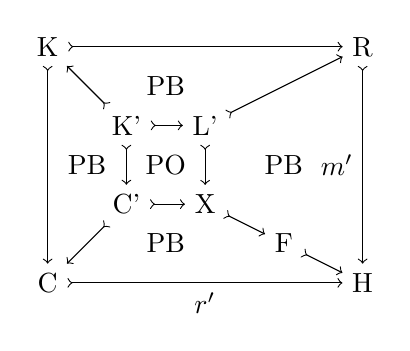
\begin{tikzpicture}
                    \node (k) at (0,0) {K};
                    \node (r) at (4,0) {R};
                    \node (c) at (0,-3) {C};
                    \node (x) at (2,-2) {X};
                    \node (h) at (4,-3) {H};
                    \node (f) at (3,-2.5) {F};
                    % \node (rb) at ($\scl*(1.5,-0.5)$) {$R_X$};
                    % \node (h') at ($\scl*(1.5,-1.5)$) {$H'$};
                    % \draw[>->]  (rb) -- (h') node [midway,above] {};
                    % \draw[>->]  (c) -- (h') node [midway,above] {};
                    \draw[<-<]  (r) -- (k) node [midway,above] {};
                    \draw[>->] (c) -- (h) node [midway, below] {$r'$};
                    \draw[>->] (r) -- (h) node[midway, left] {$m'$};
                    \draw[>->] (k) -- (c) node[midway, left] {};
                    % \draw[->] (rb) to (l);
                    % \draw[<-<] (rb) to (k);
                    \node (k') at (1,-1) {K'};
                    \node (r') at (2,-1) {L'};
                    \node (c') at (1,-2) {C'};
                    \node () at (1.5,-1.5) {PO};
                    \node () at (3,-1.5) {PB};
                    \node () at (1.5,-2.5) {PB};
                    \node () at (1.5,-0.5) {PB};
                    \node () at (0.5,-1.5) {PB};
                    % \draw [->] (x) -- (h') node[midway] {!};
                    \draw [>->] (c') -- (x);
                    \draw [>->] (r') -- (x);
                    \draw [>->] (k') -- (r');
                    \draw [>->] (k') -- (c');
                    \draw [>->] (c') -- (c);
                    % \draw [->] (h') -- (h);
                    \draw[>->] (r') -- (r) node[midway,below] {};
                    \draw[>->] (x) -- (f) node[midway,right] {};
                    \draw[>->] (f) -- (h) node[midway,right] {};
                    % \node (rb) at ($\scl*(\sclx*1.5,-0.5)$) {$R_X$};
                    % \node (h') at ($\scl*(\sclx*1.5,-1.2)$) {$H'$};
                    % \draw[>->]  (rb) -- (h') node [midway,above] {};
                    % \draw[>->]  (c) -- (h') node [midway,above] {};
                    % \draw[>->]  (rb) -- (h') node [midway,above] {};
                    % \draw[>->] (rb) to (r);
                    % \draw[<-<] (rb) to (k);
                    \draw[>->] (k') -- (k) ;
                \end{tikzpicture}
            }
            \end{center} 
    We can now construct the following commutative diagram where $L''RHF$ and $C''CHF$ are pullbacks: \todo{do we need more details?}
     \begin{center}
            \resizebox{0.3\textwidth}{!}{
                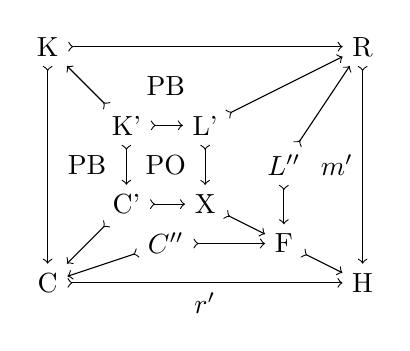
\begin{tikzpicture}
                    \node (k) at (0,0) {K};
                    \node (r) at (4,0) {R};
                    \node (c) at (0,-3) {C};
                    \node (x) at (2,-2) {X};
                    \node (h) at (4,-3) {H};
                    \node (f) at (3,-2.5) {F};
                    % \node (rb) at ($\scl*(1.5,-0.5)$) {$R_X$};
                    % \node (h') at ($\scl*(1.5,-1.5)$) {$H'$};
                    % \draw[>->]  (rb) -- (h') node [midway,above] {};
                    % \draw[>->]  (c) -- (h') node [midway,above] {};
                    \draw[<-<]  (r) -- (k) node [midway,above] {};
                    \draw[>->] (c) -- (h) node [midway, below] {$r'$};
                    \draw[>->] (r) -- (h) node[midway, left] {$m'$};
                    \draw[>->] (k) -- (c) node[midway, left] {};
                    % \draw[->] (rb) to (l);
                    % \draw[<-<] (rb) to (k);
                    \node (k') at (1,-1) {K'};
                    \node (r') at (2,-1) {L'};
                    \node (c') at (1,-2) {C'};
                    \node () at (1.5,-1.5) {PO};
                    \node (l'') at (3,-1.5) {$L''$};
                    \node (c'') at (1.5,-2.5) {$C''$};
                    \draw[>->] (c'') -- (c);
                    \draw[>->] (c'') --(f);
                    \draw[>->] (l'') --(f);
                    \draw[>->] (l'') --(r);
                    \node () at (1.5,-0.5) {PB};
                    \node () at (0.5,-1.5) {PB};
                    % \draw [->] (x) -- (h') node[midway] {!};
                    \draw [>->] (c') -- (x);
                    \draw [>->] (r') -- (x);
                    \draw [>->] (k') -- (r');
                    \draw [>->] (k') -- (c');
                    \draw [>->] (c') -- (c);
                    % \draw [->] (h') -- (h);
                    \draw[>->] (r') -- (r) node[midway,below] {};
                    \draw[>->] (x) -- (f) node[midway,right] {};
                    \draw[>->] (f) -- (h) node[midway,right] {};
                    % \node (rb) at ($\scl*(\sclx*1.5,-0.5)$) {$R_X$};
                    % \node (h') at ($\scl*(\sclx*1.5,-1.2)$) {$H'$};
                    % \draw[>->]  (rb) -- (h') node [midway,above] {};
                    % \draw[>->]  (c) -- (h') node [midway,above] {};
                    % \draw[>->]  (rb) -- (h') node [midway,above] {};
                    % \draw[>->] (rb) to (r);
                    % \draw[<-<] (rb) to (k);
                    \draw[>->] (k') -- (k) ;
                \end{tikzpicture}
            }
            \end{center} 

    Since $L''RHF$ and $C''CHF$ are pullbacks, and $L'XFHR$ and $C'CHFX$ are commutative diagrams, by the universal property of pullbacks, there are unique morphisms $h_{L'L''}:L' \rightarrowtail L''$ and $h_{C'C''}:C' \rightarrowtail C''$ such that $L'L''R$, $L'L''FX$, $C'C''FX$, and $C'CC''$ are commutative diagrams. Thus, the following diagram holds: 
    \begin{center}
            \resizebox{0.5\textwidth}{!}{
                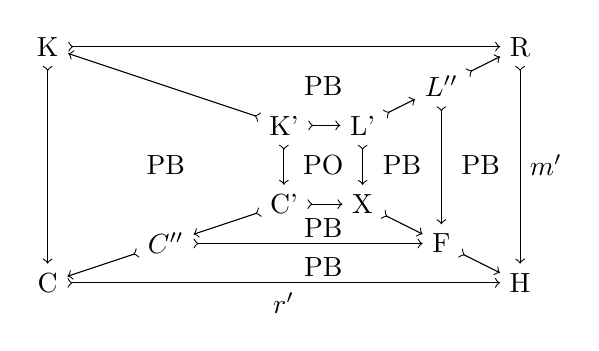
\begin{tikzpicture}
                    \node (k) at (-2,0) {K};
                    \node (r) at (4,0) {R};
                    \node (x) at (2,-2) {X};
                    \node (h) at (4,-3) {H};
                    \node (f) at (3,-2.5) {F};
                    \node (k') at (1,-1) {K'};
                    \node (r') at (2,-1) {L'};
                    \node (c) at (-2,-3) {C};
                    \node (c') at (1,-2) {C'};
                    \node (c'') at (-0.5,-2.5) {$C''$};
                    \node () at (1.5,-1.5) {PO};
                    \node () at (2.5,-1.5) {PB};
                    \node () at (3.5,-1.5) {PB};
                    \node () at (1.5,-2.3) {PB};
                    \node () at (1.5,-2.8) {PB};
                    \node (l'') at (3,-0.5) {$L''$};
                    % \node (rb) at ($\scl*(1.5,-0.5)$) {$R_X$};
                    % \node (h') at ($\scl*(1.5,-1.5)$) {$H'$};
                    % \draw[>->]  (rb) -- (h') node [midway,above] {};
                    % \draw[>->]  (c) -- (h') node [midway,above] {};
                    \draw[<-<]  (r) -- (k) node [midway,above] {};
                    \draw[>->] (c) -- (h) node [midway, below] {$r'$};
                    \draw[>->] (r) -- (h) node[midway, right] {$m'$};
                    \draw[>->] (k) -- (c) node[midway, left] {};
                    % \draw[->] (rb) to (l);
                    % \draw[<-<] (rb) to (k);
                    \draw[>->] (c'') -- (c);
                    \draw[>->] (c'') --(f);
                    \draw[>->] (l'') --(f);
                    \draw[>->] (l'') --(r);
                    \node () at (1.5,-0.5) {PB};
                    \node () at (-0.5,-1.5) {PB};
                    % \draw [->] (x) -- (h') node[midway] {!};
                    \draw [>->] (c') -- (x);
                    \draw [>->] (r') -- (x);
                    \draw [>->] (k') -- (r');
                    \draw [>->] (k') -- (c');
                    \draw [>->] (c') -- (c'');
                    % \draw [->] (h') -- (h);
                    \draw[>->] (r') -- (l'') node[midway,below] {};
                    \draw[>->] (x) -- (f) node[midway,right] {};
                    \draw[>->] (f) -- (h) node[midway,right] {};
                    % \node (rb) at ($\scl*(\sclx*1.5,-0.5)$) {$R_X$};
                    % \node (h') at ($\scl*(\sclx*1.5,-1.2)$) {$H'$};
                    % \draw[>->]  (rb) -- (h') node [midway,above] {};
                    % \draw[>->]  (c) -- (h') node [midway,above] {};
                    % \draw[>->]  (rb) -- (h') node [midway,above] {};
                    % \draw[>->] (rb) to (r);
                    % \draw[<-<] (rb) to (k);
                    \draw[>->] (k') -- (k) ;
                \end{tikzpicture}
            }
            \end{center} 

    Similarly, we can construct the following commutative diagram where $C''CKK''$ is pullback:
\begin{center}
            \resizebox{0.5\textwidth}{!}{
                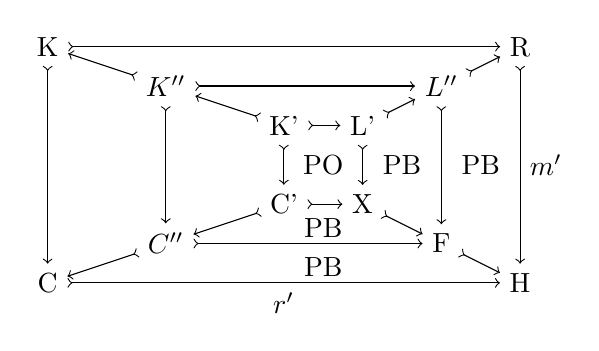
\begin{tikzpicture}
                    \node (k) at (-2,0) {K};
                    \node (r) at (4,0) {R};
                    \node (x) at (2,-2) {X};
                    \node (h) at (4,-3) {H};
                    \node (f) at (3,-2.5) {F};
                    \node (k') at (1,-1) {K'};
                    \node (r') at (2,-1) {L'};
                    \node (c) at (-2,-3) {C};
                    \node (c') at (1,-2) {C'};
                    \node (c'') at (-0.5,-2.5) {$C''$};
                    \node () at (1.5,-1.5) {PO};
                                     \node () at (2.5,-1.5) {PB};
                    \node () at (3.5,-1.5) {PB};
                    \node () at (1.5,-2.3) {PB};
                    \node () at (1.5,-2.8) {PB};
                    \node (l'') at (3,-0.5) {$L''$};
                    \node (k'') at (-0.5,-0.5) {$K''$};
                    % \node (k3) at (0,-0.66) {$K^3$};
                    \draw[>->]  (k') -- (k'') node [midway,above] {};
                    % \draw[>->]  (k3) -- (k2) node [midway,above] {};
                    \draw[>->]  (k'') -- (k) node [midway,above] {};
                    \draw[>->]  (k'') -- (c'') node [midway,above] {};
                    \draw[>->]  (k'') -- (l'') node [midway,above] {};
                    % \node (rb) at ($\scl*(1.5,-0.5)$) {$R_X$};
                    % \node (h') at ($\scl*(1.5,-1.5)$) {$H'$};
                    % \draw[>->]  (rb) -- (h') node [midway,above] {};
                    % \draw[>->]  (c) -- (h') node [midway,above] {};
                    \draw[<-<]  (r) -- (k) node [midway,above] {};
                    \draw[>->] (c) -- (h) node [midway, below] {$r'$};
                    \draw[>->] (r) -- (h) node[midway, right] {$m'$};
                    \draw[>->] (k) -- (c) node[midway, left] {};
                    % \draw[->] (rb) to (l);
                    % \draw[<-<] (rb) to (k);
                    \draw[>->] (c'') -- (c);
                    \draw[>->] (c'') --(f);
                    \draw[>->] (l'') --(f);
                    \draw[>->] (l'') --(r);
                    % \node () at (1.5,-0.5) {PB};
                    % \node () at (-0.5,-1.5) {PB};
                    % \draw [->] (x) -- (h') node[midway] {!};
                    \draw [>->] (c') -- (x);
                    \draw [>->] (r') -- (x);
                    \draw [>->] (k') -- (r');
                    \draw [>->] (k') -- (c');
                    \draw [>->] (c') -- (c'');
                    % \draw [->] (h') -- (h);
                    \draw[>->] (r') -- (l'') node[midway,below] {};
                    \draw[>->] (x) -- (f) node[midway,right] {};
                    \draw[>->] (f) -- (h) node[midway,right] {};
                    % \node (rb) at ($\scl*(\sclx*1.5,-0.5)$) {$R_X$};
                    % \node (h') at ($\scl*(\sclx*1.5,-1.2)$) {$H'$};
                    % \draw[>->]  (rb) -- (h') node [midway,above] {};
                    % \draw[>->]  (c) -- (h') node [midway,above] {};
                    % \draw[>->]  (rb) -- (h') node [midway,above] {};
                    % \draw[>->] (rb) to (r);
                    % \draw[<-<] (rb) to (k);
                    % \draw[>->] (k') -- (k) ;
                \end{tikzpicture}
            }
            \end{center} 

   


    % There exists $h_{L'L''}:L' \rightarrowtail L''$ such that $h_{L'L} = h_{L'L''} \star h_{L''L}$ 
    % because $L''LGF$ is a pullback, and the following diagram holds:



    % \begin{center}
    %     \resizebox{0.3\textwidth}{!}{
    %         \begin{tikzpicture}
    %             \node (k) at (0,0) {K};
    %             \node (r) at (4,0) {L};
    %             \node (c) at (0,-3) {C};
    %             \node (h) at (4,-3) {G};
    %             \draw[<-<]  (r) -- (k) node [midway,above] {};
    %             \draw[>->] (c) -- (h) node [midway, below] {};
    %             \draw[>->] (r) -- (h) node[midway, left] {m};
    %             \draw[>->] (k) -- (c) node[midway, left] {};
    %             \node (k') at (1,-1) {K'};
    %             \node (r') at (2,-1) {L'};
    %             \node (c') at (1,-2) {C'};
    %             \node () at (1.5,-1.5) {PO};
    %             \node () at (3,-1.5) {PB};
    %             \node () at (1.5,-2.5) {PB};
    %             \node () at (1.5,-0.5) {PB};
    %             \node () at (0.5,-1.5) {PB};
    %             \node (x) at (2,-2) {X};
    %             \draw [>->] (c') -- (x);
    %             \draw [>->] (r') -- (x);
    %             \draw [>->] (k') -- (r');
    %             \draw [>->] (k') -- (c');
    %             \draw [>->] (c') -- (c);
    %             \draw[>->] (r') -- (r);
    %             \draw[>->] (x) -- (h) node[midway,right] {};
    %             \draw[>->] (k') -- (k) ;
    %         \end{tikzpicture}
    %     }
    %     \end{center} 
    % where
    % \begin{flalign*}
    %     h_{L'L} \star m &= h_{L'X} \star h_{XG} \\
    %                     &= h_{L'X} \star h_{XF} \star h_{FG}
    %                     &\text{by~\eqref{antipattern:eq:xxxhxg}}
    % \end{flalign*} 
    % Analogously, there exist $h_{C'C''}:C' \rightarrowtail C''$ such that $h_{C'C} = h_{C'C''} \star h_{C''C}$ 
    % and $h_{K'K''}:K' \rightarrowtail K''$ such that $h_{K'K} = h_{K'K''} \star h_{K''K}$.
    
     \todo{details}We can show that the following diagram holds:

    \begin{center}
        \resizebox{0.3\textwidth}{!}{
            \begin{tikzpicture}
                \node (kk) at (-1,1) {K};
                \node (rr) at (5,1) {R};
                \node (cc) at (-1,-4) {C};
                \node (hh) at (5,-4) {H};
                \node (k) at (0,0) {K''};
                \node (r) at (4,0) {L''};
                \node (c) at (0,-3) {C''};
                \node (h) at (4,-3) {F};
                \draw[>->]  (k) -- (kk) node [midway,above] {};
                \draw[>->]  (c) -- (cc) node [midway,above] {};
                \draw[>->]  (h) -- (hh) node [midway,above] {};
                \draw[>->]  (r) -- (rr) node [midway,above] {};
                \draw[>->]  (cc) -- (hh) node [midway,below] {$r'$};
                \draw[>->]  (kk) -- (cc) node [midway,left] {$u$};
                \draw[>->]  (kk) -- (rr) node [midway,above] {$r$};
                \draw[>->]  (rr) -- (hh) node [midway,right] {$m'$};
                % \node (rb) at ($\scl*(1.5,-0.5)$) {$R_X$};
                % \node (h') at ($\scl*(1.5,-1.5)$) {$H'$};
                % \draw[>->]  (rb) -- (h') node [midway,above] {};
                % \draw[>->]  (c) -- (h') node [midway,above] {};
                \draw[<-<]  (r) -- (k) node [midway,above] {};
                \draw[>->] (c) -- (h) node [midway, below] {};
                \draw[>->] (r) -- (h) node[midway, left] {};
                \draw[>->] (k) -- (c) node[midway, left] {};
                % \draw[->] (rb) to (l);
                % \draw[<-<] (rb) to (k);
                \node (k') at (1,-1) {K'};
                \node (r') at (2,-1) {L'};
                \node (c') at (1,-2) {C'};
                \node () at (1.5,-1.5) {PO};
                \node () at (3,-1.5) {PB};
                \node () at (1.5,-2.5) {PB};
                \node () at (1.5,-0.5) {PB};
                \node () at (0.5,-1.5) {PB};
                \node () [at=($(cc)!0.5!(h)$)] {PB};
                \node () [at=($(cc)!0.5!(k)$)] {PB};
                \node () [at=($(rr)!0.5!(k)$)] {PB};
                \node () [at=($(rr)!0.5!(h)$)] {PB};
                \node (x) at (2,-2) {X};
                % \draw [->] (x) -- (h') node[midway] {!};
                \draw [>->] (c') -- (x);
                \draw [>->] (r') -- (x);
                \draw [>->] (k') -- (r');
                \draw [>->] (k') -- (c');
                \draw [>->] (c') -- (c);
                % \draw [->] (r') -- (rb);
                % \draw [->] (r') -- (rb);
                % \draw [->] (h') -- (h);
                \draw[>->] (r') -- (r) node[midway,below] {};
                \draw[>->] (x) -- (h) node[midway,right] {};
                % \node (rb) at ($\scl*(\sclx*1.5,-0.5)$) {$R_X$};
                % \node (h') at ($\scl*(\sclx*1.5,-1.2)$) {$H'$};
                % \draw[>->]  (rb) -- (h') node [midway,above] {};
                % \draw[>->]  (c) -- (h') node [midway,above] {};
                % \draw[>->]  (rb) -- (h') node [midway,above] {};
                % \draw[>->] (rb) to (r);
                % \draw[<-<] (rb) to (k);
                \draw[>->] (k') -- (k) ;
            \end{tikzpicture}
        }
        \end{center} 
        % Hyp ?? $h_{L'R} = Id_{L'L''} \star h_{L''R}$ !!\\
        We have $h_{XH} = h_{XF} \star h_{FH}$ because $K'C'XL'$ is a pushout and $h_{XH}$ 
        is the unique morphism such that $H_{C'X} \star h_{XH} = h_{C'C} \star h_{CH} =  h_{C'C''} \star h_{C''C} \star h_{CH}$ and 
        $h_{L'X} \star h_{XH} = h_{L'R} \star h_{RH} = h_{L'L''} \star h_{L''R} \star h_{RH}$, but we have 
        \begin{flalign*}
            &h_{C'X} \star (h_{XF} \star h_{FH}) 
            \\= & (h_{C'C''} \star h_{C''F}) \star h_{FH} 
            \\= & h_{C'C''} \star (h_{C''C} \star h_{CH})
        \end{flalign*}
        and 
        \begin{flalign*}
            &h_{L'X} \star (h_{XF} \star h_{FH})
            \\ = & (h_{L'L''} \star h_{L''F}) \star h_{FH}
            \\ = & h_{L'L''} \star (h_{L''R} \star h_{RH})
        \end{flalign*}
        This concludes our proof.
\end{proof}


% \begin{lemma}
%     \label{lem:w_g_geq_w_h_leq}
%     Let $\rho = (L \overset{l}{\leftarrowtail} K \overset{r}{\rightarrowtail} R)$ be an injective DPO rewriting rule,
%     \( (X, \emptyset) \) a ruler-graph,
%     and \( G \Rightarrow_{\rho,\mathfrak{M}} H \) a rewriting step. 
%     If $\rho$ is ?? then:\[
%         |Mono(\mathcal{X},G)_{NF}| - |Mono(\mathcal{X},H)_{NF}|
%         \geq 
%         |Mono(X,L)| - |Mono(X,R)|
%     \]
% \end{lemma}
% \begin{proof}
%     \label{proof:lem:w_g_geq_w_h_leq}
%     Let the following diagram be the witness diagram of the rewriting step
%     \begin{center}
%         \begin{tikzpicture}
%             \node (k) at (0,1) {K};
%             \node (l) at (-2,1) {L};
%             \node (r) at (2,1) {R};
%             \node (c) at (0,-1) {C};
%             \node (g) at (-2,-1) {G};
%             \node (h) at (2,-1) {H};
%             \draw[<-<]  (l) -- (k) node [midway,below] {l};
%             \draw[>->]  (k) -- (r) node [midway,below] {r};
%             \draw[>->] (c) -- (g) node [midway, above] {l'};
%             \draw[>->] (c) -- (h) node [midway,above] {r'};
%             \draw[>->] (l) -- (g) node[midway, right] {m};
%             \draw[>->] (r) -- (h) node[midway, left] {m'};
%             \draw[>->] (k) -- (c) node[midway, left] {};
%             \node () [at=($(l)!0.5!(c)$)] {PO};
%             \node () [at=($(r)!0.5!(c)$)] {PO};
%         \end{tikzpicture}
%     \end{center}
%     We have 
%     \begin{flalign*}
%         &\card{\operatorname{Mono}(X,G)_{NF}} 
%         = & \card{\operatorname{Mono}(X,G)}
%             % \overset{\operatorname{def}}{=} 
%             % w_{T_\Sigma}(t_G) 
%         \\
%         % =& \Psi_{G}\\
%         =& 
%         \card{\operatorname{Mono}(X,G,l')
%         \uplus
%          \operatorname{Mono}(X,G,\lnot l',m)
%         \uplus
%          \operatorname{Mono}(X,G,\lnot l',\lnot m)}\\
%         =& 
%         \card{\operatorname{Mono}(X,G,l')}
%         +
%         \textcolor{red}{\card{\operatorname{Mono}(X,G,\lnot l',m)}}
%         +
%         \card{\operatorname{Mono}(X,G,\lnot l',\lnot m)}
%         \\
%     =& \card{\operatorname{Mono}(X,C)}
%             +
%             \card{\operatorname{Mono}(X, L, \lnot l)} 
%             +
%             \card{\operatorname{Mono}(X, G,\lnot l', \lnot m)} 
%         &  \text{by~\autoref{lem:decomp_w_u}}
%     \end{flalign*}
%     and
%     \begin{flalign*}
%         % ligne 1
%         &\card{\operatorname{Mono}(X,H)_{NF}}
%         = &\card{\operatorname{Mono}(X,H)}
%         % \overset{\operatorname{def}}{=}  
%         %     w_{T_\Sigma}(t_H )
%         \\
%         =& 
%         \card{\operatorname{Mono}(X,H,r')
%         \uplus
%             \operatorname{Mono}(X,H,\lnot r',m')
%         \uplus
%             \operatorname{Mono}(X,H,\lnot r',\lnot m')}
%         \\
%         =& 
%         \card{\operatorname{Mono}(X,H,r')}
%         +
%         \textcolor{red}{\card{\operatorname{Mono}(X,H,\lnot r',m')}}
%         +
%         \card{\operatorname{Mono}(X,H,\lnot r',\lnot m')}
%         \\
%         % = & \Psi_{H} \\
%         % ligne 2
%         = &
%             \card{\operatorname{Mono}(X,C)}
%             +
%             \card{\operatorname{Mono}(X, R, \lnot r)} 
%             +
%             \card{\operatorname{Mono}(X, H, \lnot r', \lnot m')}
%         % ( 
%         %             w_{T_\Sigma} (h_{RH} \star t_H ) + w_{T_\Sigma} (h_{CH} \star t_H  -h_{KC}) 
%         % )
%         %         +  w_{T_\Sigma}(t_H  - \{h_{RH},h_{CH} \})  
%         &  \text{by~\autoref{lem:decomp_w_u}}
%     \end{flalign*}
%     Therefore, the following inequality holds
%      \begin{flalign*}
%            &\card{\operatorname{Mono}(X,G)} - \card{\operatorname{Mono}(X,H)} &\\
%            =&(\card{\operatorname{Mono}(X, L, \lnot l)} - \card{\operatorname{Mono}(X, R, \lnot r)}) + 
%            \textcolor{red}{(\card{\operatorname{Mono}(X, G, \lnot l', \lnot m)} - \card{\operatorname{Mono}(X, H, \lnot r', \lnot m')})}  \\
%        \geq& \textcolor{red}{\card{\operatorname{Mono}(X, L, \lnot l)} - \card{\operatorname{Mono}(X, R, \lnot r)}} \hspace{3cm} \text{by~\autoref{lem:w_u_l_not_geq_r_not}} \\
%           =& \card{\operatorname{Mono}(X, L)} - \card{\operatorname{Mono}(X, R)} \hspace{3cm} \text{by~\autoref{lem:xlnlmxrnr}}
%      \end{flalign*}
% \end{proof}

 
% \begin{lemma}
%     \label{lem:w_g_geq_w_h_leq_with_forbidden_contexts}
%     Let $\rho = (L \overset{l}{\leftarrowtail} K \overset{r}{\rightarrowtail} R)$ be an injective DPO rewriting rule,
%     \( (X, F_X) \) a ruler-graph,
%     and \( G \Rightarrow_{\rho,\mathfrak{M}} H \) a rewriting step. 
%     If $\rho$ is ?? then:\[
%         |Mono(\mathcal{X},G)_{NF}| - |Mono(\mathcal{X},H)_{NF}|
%         \geq 
%         |Mono(X,L)| - |Mono(X,R)|
%     \]
% \end{lemma}
% \begin{proof}
%     \label{proof:lem:w_g_geq_w_h_leq_with_forbidden_contexts}
%     Let the following diagram be the witness diagram of the rewriting step
%     \begin{center}
%         \begin{tikzpicture}
%             \node (k) at (0,1) {K};
%             \node (l) at (-2,1) {L};
%             \node (r) at (2,1) {R};
%             \node (c) at (0,-1) {C};
%             \node (g) at (-2,-1) {G};
%             \node (h) at (2,-1) {H};
%             \draw[<-<]  (l) -- (k) node [midway,below] {l};
%             \draw[>->]  (k) -- (r) node [midway,below] {r};
%             \draw[>->] (c) -- (g) node [midway, above] {l'};
%             \draw[>->] (c) -- (h) node [midway,above] {r'};
%             \draw[>->] (l) -- (g) node[midway, right] {m};
%             \draw[>->] (r) -- (h) node[midway, left] {m'};
%             \draw[>->] (k) -- (c) node[midway, left] {};
%             \node () [at=($(l)!0.5!(c)$)] {PO};
%             \node () [at=($(r)!0.5!(c)$)] {PO};
%         \end{tikzpicture}
%     \end{center}
%     We have 
%     \begin{flalign*}
%         &\card{\operatorname{Mono}(X,G)_{NF}} 
%         = & \card{\operatorname{Mono}(X,G)}
%             % \overset{\operatorname{def}}{=} 
%             % w_{T_\Sigma}(t_G) 
%         \\
%         % =& \Psi_{G}\\
%         =& 
%         \card{\operatorname{Mono}(X,G,l')
%         \uplus
%          \operatorname{Mono}(X,G,\lnot l',m)
%         \uplus
%          \operatorname{Mono}(X,G,\lnot l',\lnot m)}\\
%         =& 
%         \card{\operatorname{Mono}(X,G,l')}
%         +
%         \textcolor{red}{\card{\operatorname{Mono}(X,G,\lnot l',m)}}
%         +
%         \card{\operatorname{Mono}(X,G,\lnot l',\lnot m)}
%         \\
%     =& \card{\operatorname{Mono}(X,C)}
%             +
%             \card{\operatorname{Mono}(X, L, \lnot l)} 
%             +
%             \card{\operatorname{Mono}(X, G,\lnot l', \lnot m)} 
%         &  \text{by~\autoref{lem:decomp_w_u}}
%     \end{flalign*}
%     and
%     \begin{flalign*}
%         % ligne 1
%         &\card{\operatorname{Mono}(X,H)_{NF}}
%         = &\card{\operatorname{Mono}(X,H)}
%         % \overset{\operatorname{def}}{=}  
%         %     w_{T_\Sigma}(t_H )
%         \\
%         =& 
%         \card{\operatorname{Mono}(X,H,r')
%         \uplus
%             \operatorname{Mono}(X,H,\lnot r',m')
%         \uplus
%             \operatorname{Mono}(X,H,\lnot r',\lnot m')}
%         \\
%         =& 
%         \card{\operatorname{Mono}(X,H,r')}
%         +
%         \textcolor{red}{\card{\operatorname{Mono}(X,H,\lnot r',m')}}
%         +
%         \card{\operatorname{Mono}(X,H,\lnot r',\lnot m')}
%         \\
%         % = & \Psi_{H} \\
%         % ligne 2
%         = &
%             \card{\operatorname{Mono}(X,C)}
%             +
%             \card{\operatorname{Mono}(X, R, \lnot r)} 
%             +
%             \card{\operatorname{Mono}(X, H, \lnot r', \lnot m')}
%         % ( 
%         %             w_{T_\Sigma} (h_{RH} \star t_H ) + w_{T_\Sigma} (h_{CH} \star t_H  -h_{KC}) 
%         % )
%         %         +  w_{T_\Sigma}(t_H  - \{h_{RH},h_{CH} \})  
%         &  \text{by~\autoref{lem:decomp_w_u}}
%     \end{flalign*}
%     Therefore, the following inequality holds
%      \begin{flalign*}
%            &\card{\operatorname{Mono}(X,G)} - \card{\operatorname{Mono}(X,H)} &\\
%            =&(\card{\operatorname{Mono}(X, L, \lnot l)} - \card{\operatorname{Mono}(X, R, \lnot r)}) + 
%            \textcolor{red}{(\card{\operatorname{Mono}(X, G, \lnot l', \lnot m)} - \card{\operatorname{Mono}(X, H, \lnot r', \lnot m')})}  \\
%        \geq& \textcolor{red}{\card{\operatorname{Mono}(X, L, \lnot l)} - \card{\operatorname{Mono}(X, R, \lnot r)}} \hspace{3cm} \text{by~\autoref{lem:w_u_l_not_geq_r_not}} \\
%           =& \card{\operatorname{Mono}(X, L)} - \card{\operatorname{Mono}(X, R)} \hspace{3cm} \text{by~\autoref{lem:xlnlmxrnr}}
%      \end{flalign*}
%     \qed
% \end{proof}



\noindent
\begin*{\textbf{\autoref{antipattern:thm:termination_grs}}}(Termination)

Let \(\mathcal{A}\) and \(\mathcal{B}\) be sets of injective DPO rewriting rules, $\mathbb{X}$ a set of ruler-graphs and $s_\mathbb{X}$ a weight function. If the following hold:
\begin{enumerate}
    \item\label{antipattern:thm:termination_grs:assump:1}  for every $\rho \in \mathcal{A} \cup \mathcal{B}$ and for every \( \mathcal{X} \in \mathbb{X} \) with underlying graph $X$, 
        % the number of $X$-occurrences that are not included in any occurrences of the forbidden context $F \in F_x$ in a $\rho$-rewriting step is predictable,
        $\rho$ is $X$-non-increasing, and if $\mathcal{X}= (X,f:X \rightarrowtail F)$ then $\rho^{-1}$ is $X$-non-increasing and $F$-non-increasing,
        % $\rho^{-1}$ is $F$-non-increasing if $\mathcal{X}= (X,f:X \rightarrowtail F)$ and, $\rho$ and $\rho^{-1}$ are $X$-non-increasing
    \item\label{antipattern:thm:termination_grs:assump:2}  for every \(\rho \in \mathcal{A}\), 
    % \( w_{s_\mathbb{X}}(lhs(\rho)) > w_{s_\mathbb{X}}(rhs(\rho)) \),
    \( \sum_{\mathcal{X} \in \mathbb{X}}^{}s_\mathbb{X}(X) * \left( 
        \card{\operatorname{Mono}(X,L)} -
        \card{\operatorname{Mono}(X,R)}
        \right) > 0 \),
    \item\label{antipattern:thm:termination_grs:assump:3}  for every \(\rho \in \mathcal{B}\),  
    % \( w_{s_\mathbb{X}}(lhs(\rho)) \geq w_{s_\mathbb{X}}(rhs(\rho)) \).
    \( \sum_{\mathcal{X} \in \mathbb{X}}^{}s_\mathbb{X}(X) * \left( 
        \card{\operatorname{Mono}(X,L)} -
        \card{\operatorname{Mono}(X,R)}
        \right) \geq 0 \).
\end{enumerate}
Then \(\Rightarrow_{\mathcal{A},\mathcal{M}}\) is terminating relative to \(\Rightarrow_{\mathcal{B},\mathcal{M}}\).
\end*{}


% Let \(\mathcal{A}\) and \(\mathcal{B}\) be sets of injective DPO rewriting rules, $\mathbb{X}$ a set of ruler-graphs and $s_\mathbb{X}$ a weight function. If the following hold:
%     \begin{enumerate}
%         \item  for every $\rho \in \mathcal{A} \cup \mathcal{B}$ and for every \( \mathcal{X} \in \mathbb{X} \) with underlying graph $X$, 
%         % the number of $X$-occurrences that are not included in any occurrences of the forbidden context $F \in F_x$ in a $\rho$-rewriting step is predictable,
%         $\rho$ is $X$-non-increasing, and if $\mathcal{X}= (X,f:X \rightarrowtail F)$ then $\rho^{-1}$ is $X$-non-increasing and $F$-non-increasing,
%         % $\rho^{-1}$ is $F$-non-increasing if $\mathcal{X}= (X,f:X \rightarrowtail F)$ and, $\rho$ and $\rho^{-1}$ are $X$-non-increasing
%         \item for every \(\rho \in \mathcal{A}\), we have
%         % \( w_{s_\mathbb{X}}(lhs(\rho)) > w_{s_\mathbb{X}}(rhs(\rho)) \),
%         $ \sum_{\mathcal{X} \in \mathbb{X}}^{}s_\mathbb{X}(X) * 
%             \Lambda(\mathcal{X},\rho) > 0 $
%         \item for every \(\rho \in \mathcal{B}\), we have   
%         % \( w_{s_\mathbb{X}}(lhs(\rho)) \geq w_{s_\mathbb{X}}(rhs(\rho)) \).
%         $ 
%             \sum_{\mathcal{X} \in \mathbb{X}}^{}s_\mathbb{X}(X) * \Lambda(\mathcal{X},\rho) \geq 0 
%         $
%     \end{enumerate}
%     Then \(\Rightarrow_{\mathcal{A},\mathcal{M}}\) is terminating relative to \(\Rightarrow_{\mathcal{B},\mathcal{M}}\).

\begin{proof} 
    \label{antipattern:proof:thm:termination_grs}
    
    By Assumption~\eqref{antipattern:thm:termination_grs:assump:1} and~\autoref{antipattern:lem:w_g_geq_w_h_leq}, the inequality \(
        w_{s_\mathbb{X}}(G) - w_{s_\mathbb{X}}(H) 
        \geq 
        \sum_{\mathcal{X} \in \mathbb{X}}^{}s_\mathbb{X}(X) * \left( 
            \card{\operatorname{Mono}(X,L)} -
            \card{\operatorname{Mono}(X,R)}
            \right)
    \) holds for all rewriting steps $G \Rightarrow_{\rho, \mathcal{M}} H$  with $\rho \in \mathcal{A} \cup \mathcal{B}$.
    
    \noindent From Assumption~\eqref{antipattern:thm:termination_grs:assump:2} and Assumption~\eqref{antipattern:thm:termination_grs:assump:3}, we deduce 
    \begin{itemize}
        \item \( w_{s_\mathbb{X}}(G) > w_{s_\mathbb{X}}(H) \) for every rule \(\rho \in \mathcal{A}\);
        \item  \( w_{s_\mathbb{X}}(G) \geq w_{s_\mathbb{X}}(H) \) for every rule \(\rho \in \mathcal{B}\).
    \end{itemize}
    Since $w_{s_\mathbb{X}}(G) \in \mathbb{N}$ for all graph $G$. Every rewriting sequence can only have a finite number of rewriting steps using rules in $\mathcal{A}$.
\end{proof} 